
%% Uncomment one of these:
%% the 1st when using pdflatex, which directly typesets your document in
%% pdf (use jpg or pdf figures), or
%% the 2nd when producing a ps file (use eps figures, don't use ps figures!).
\documentclass[english,12pt,a4paper,pdftex,elec,utf8]{aaltothesis}
%\documentclass[english,12pt,a4paper,dvips]{aaltothesis}

%% To the \documentclass above
%% specify your school: arts, biz, chem, elec, eng, sci
%% specify the character encoding scheme used by your editor: utf8, latin1

%% Use one of these if you write in Finnish (see the Finnish template):
%%
%\documentclass[finnish,12pt,a4paper,pdftex,elec,utf8]{aaltothesis}
%\documentclass[finnish,12pt,a4paper,dvips]{aaltothesis}

\usepackage{graphicx}
%% Use this if you write hard core mathematics, these are usually needed
\usepackage{amsfonts,amssymb,amsbsy}

%% Use the macros in this package to change how the hyperref package below 
%% typesets its hypertext -- hyperlink colour, font, etc. See the package
%% documentation. It also defines the \url macro, so use the package when 
%% not using the hyperref package.
%%
%\usepackage{url}

%% Use this if you want to get links and nice output. Works well with pdflatex.
\usepackage{hyperref}
\hypersetup{pdfpagemode=UseNone, pdfstartview=FitH,
  colorlinks=true,urlcolor=red,linkcolor=blue,citecolor=black,
  pdftitle={Offline Trajectory Metrics for Early Stopping in Vision-Language-Action Model Fine-Tuning},
  pdfauthor={Yibo Zhang},
  pdfkeywords={Vision-Language-Action models, early stopping, offline policy evaluation, fine-tuning}}

%% For flow chart
% \documentclass{article}
\usepackage{tikz}
\usepackage{float}
\usetikzlibrary{positioning, arrows.meta, shapes.geometric, shadows, calc, matrix}

\usepackage{gensymb}
\usetikzlibrary{shapes.geometric, arrows}

%% For aligned equal
\usepackage{amsmath}
\usepackage{booktabs}

\usepackage{tikz}
\usetikzlibrary{arrows.meta, positioning}

%% for terminal style output.
\usepackage{listings}
\usepackage{xcolor}
% \usepackage[scaled]{beramono}  % optional: better monospace font
%\definecolor{lightgray}{gray}{0.95}
\lstdefinestyle{terminal}{
  backgroundcolor=\color{lightgray},
  basicstyle=\ttfamily\footnotesize,
  frame=single,
  breaklines=true,
  showstringspaces=false,
  columns=fullflexible,
}

%% Shorthand macros used in the optimization equations
\newcommand{\Loss}{\mathcal{L}}
\newcommand{\mhat}{\hat{m}}
\newcommand{\vhat}{\hat{v}}

\usepackage{cite}  % Or use \usepackage{biblatex} if you prefer
\usepackage{natbib}
\bibliographystyle{ieeetr}

%% All that is printed on paper starts here
\begin{document}

%% Change the school field to specify your school if the automatically 
%% set name is wrong
% \university{aalto-yliopisto}
\university{Aalto University}
% \school{Sähkötekniikan korkeakoulu}
\school{School of Electrical Engineering}

%% Only for B.Sc. thesis: Choose your degree programme. 
%\degreeprogram{Electronics and electrical engineering}
%%

%% ONLY FOR M.Sc. AND LICENTIATE THESIS: Specify your department,
%% professorship and professorship code. 
%%
\department{Department of Electrical Engineering and Automation}
\professorship{Aalto Robot Learning Lab}
%%

%% Valitse yksi näistä kolmesta
%%
%% Choose one of these:
%\univdegree{BSc}
\univdegree{MSc}
%\univdegree{Lic}

%% Your own name (should be self explanatory...)
\author{Yibo Zhang}

%% Your thesis title comes here and again before a possible abstract in
%% Finnish or Swedish . If the title is very long and latex does an
%% unsatisfactory job of breaking the lines, you will have to force a
%% linebreak with the \\ control character. 
%% Do not hyphenate titles.
%% 
\thesistitle{Offline Trajectory Metrics for Early Stopping in Vision-Language-Action Model Fine-Tuning}

\place{Espoo}

%% For B.Sc. thesis use the date when you present your thesis. 
%% 
%% Kandidaatintyön päivämäärä on sen esityspäivämäärä! 
\date{21.7.2026}

%% B.Sc. or M.Sc. thesis supervisor 
%% Note the "\" after the comma. This forces the following space to be 
%% a normal interword space, not the space that starts a new sentence. 
%% This is done because the fullstop isn't the end of the sentence that
%% should be followed by a slightly longer space but is to be followed
%% by a regular space.
%%
\supervisor{Prof.\ Joni Pajarinen} 

%% B.Sc. or M.Sc. thesis advisors(s). You can give upto two advisors in
%% this template. Check with your supervisor how many official advisors
%% you can have.
%%
%\advisor{Prof.\ Pirjo Professori}
\advisor{Dr. Wenyan Yang}
%\advisor{M.Sc.\ Polli Pohjaaja}

%% Aalto logo: syntax:
%% \uselogo{aaltoRed|aaltoBlue|aaltoYellow|aaltoGray|aaltoGrayScale}{?|!|''}
%%
%% Logo language is set to be the same as the document language.
%% Logon kieli on sama kuin dokumentin kieli
%%
\uselogo{aaltoYellow}{!}

%% Create the coverpage
%%
\makecoverpage


%% Note that when writting your master's thesis in English, place
%% the English abstract first followed by the possible Finnish abstract

%% English abstract.
%% All the information required in the abstract (your name, thesis title, etc.)
%% is used as specified above.
%% Specify keywords
%%
%% Kaikki tiivistelmässä tarvittava tieto (nimesi, työnnimi, jne.) käytetään
%% niin kuin se on yllä määritelty.
%% Avainsanat
%%
\keywords{Vision-Language-Action models, early stopping, offline policy evaluation, trajectory similarity metrics, imitation learning}
%% Abstract text
\begin{abstractpage}[english]

Vision-Language-Action models (VLAs) are typically fine-tuned for a fixed number of training steps without an explicit validation-based stopping criterion, because training loss is a poor proxy for closed-loop task performance and online rollout evaluation is too expensive to run at every checkpoint. This work benchmarks offline validation metrics as early-stopping signals for VLA fine-tuning across five LoRA fine-tuning runs of three VLA architectures --- the discrete-token OpenVLA, the flow-matching SmolVLA and $\pi_{0.5}$ --- to evaluate which metric best predicts closed-loop success without requiring a real or simulated rollout at every checkpoint. Each metric is scored against closed-loop success rate by rank correlation, selection regret, and bootstrap confidence interval. Trajectory-similarity metrics correlate positively with closed-loop success in every run, outperform likelihood-based surrogates on the flow-matching architectures, reliably identify the converged training region, and support low-regret early-stopping checkpoint selection. In addition, the same offline metrics are extended from the checkpoint to a deployment-time hyperparameter, the open-loop horizon over which a predicted action chunk is executed before the policy replans: under a fixed-window construction, they are significantly effective at selecting a low-regret horizon, though the best-suited metric for this decision differs from the one recommended for checkpoint selection.
\end{abstractpage}


%% Preface
%%
%% Esipuhe 
\mysection{Preface}
%\mysection{Esipuhe}
Robotics and control have been a lifelong dream, ever since my first LOGO-programmed turtle drew a square on the screen. That moment sparked my passion, and I have pursued it throughout my student years. At age eight, I programmed a sensor-equipped smart car to navigate a maze. As an undergraduate, I threw myself into electronic design with great enthusiasm and developed my own autonomous drone fleets, gradually entering the field of machine learning. During my studies abroad in Finland and Germany, I entered the domain of deep learning and autonomous driving, and had the opportunity to work with state-of-the-art VLA models for my master's thesis topic, and get a great job as an autonomous drone research scientist. I am closer to my robotics dream than ever before—one that aligns seamlessly with my personal interests, career aspirations, current job scope, and the broader trajectory of the embedded AI era.

I have been incredibly fortunate to have Prof. Joni Pajarinen, Dr. Wenyan Yang, and Dr. Aidan Scannell for offering me this interesting research topic, guiding me into the field, providing experimental suggestions, and pushing me forward whenever I hit a roadblock. During our meetings, just a few sentences from them could shed light on challenges that had troubled me for days or even weeks. Thank you very much!

My deepest thanks go to my Dad and Mom for providing solid support to me throughout my studies abroad, financially, emotionally, and in terms of life wisdom. I am grateful to my girlfriend, Zixuan Ning, for her companionship, for sharing both the joys and challenges of life, and for striving together on the path of studying and academic pursuits. I am also grateful to my work supervisor, Prof. Eija Honkavaara, for offering me the wonderful opportunity to work on drone projects with SOTA algorithms, for understanding and supporting me in many aspects, and for serving as a role model in both academics and career.

Lastly, the biggest thanks go to myself—for staying deeply motivated in this topic, actively learning new subjects, diligently debugging countless hardware and software details, and for pulling through every challenge, stress, and torment from various aspects. No pain, no gain. Finally, I am ready for the next stage.

Through this period of thesis work, I have gained several profound insights and reflections. First, active interaction is crucial. It is often more practical to take small, iterative steps and adjust based on feedback than to attempt a single, perfect stride all at once. Even the most meticulous plan must be actively adapted to external factors. This is, in some ways, similar to the model training in this thesis: no matter how advanced the algorithm, there is invariably a gap between the predicted estimates and the actual ground truth. Greater interaction helps us better understand the real-world situation and respond accordingly.

Second, don't let physical diligence mask mental laziness, nor let technical superiority camouflage tactical foolishness. Like model training, simply extending training steps or piling up GPU resources without digging into the root cause of an issue will not truly solve it. As a consequence, such an approach merely wastes time, drains energy, and squanders valuable opportunities.

Third, focus on only one thing at a time. Attention is a finite resource. When plans conflict with changing realities, take a step back, reflect on your true thoughts, rebalance your inner world, and then commit firmly to the goal that you genuinely hold and truly want to pursue.

Last but not least, stay physically active—it is the bare minimum for maintaining resilience and achieving a flow state. As the slogan of my favorite running gear brand says, a sound mind resides in a sound body.
\\

\vspace{5cm}
Otaniemi, 21.7.2026

\vspace{5mm}
{\hfill Yibo Zhang \hspace{1cm}}

%% Force new page after preface
%%
%% Pakotetaan varmuuden vuoksi esipuheen jälkeinen osa
%% alkamaan uudelta sivulta
\newpage


%% Table of contents. 
\thesistableofcontents


%% Symbols and abbreviations
\mysection{Symbols and abbreviations}

\subsection*{Symbols}

\begin{tabular}{ll}
$k$                              & training-step / checkpoint index \\
$\theta_k$                       & policy parameters at checkpoint $k$ \\
$\pi_k = \pi_{\theta_k}$         & policy at checkpoint $k$ \\
$o_t,\,h_t$                      & observation / policy input at time $t$ \\
$a_t$                            & robot action at time $t$ \\
$H$                              & action-chunk horizon \\
$A^\star,\,A_k$                  & expert / predicted action chunk of horizon $H$ \\
$\mathcal{D},\,\mathcal{D}_{\mathrm{train}},\,\mathcal{D}_{\mathrm{val}},\,\mathcal{D}_{\mathrm{test}}$ & full dataset and its train/validation/test splits \\
$D_{\mathrm{DTW}},\,D_{\mathrm{OT}},\,D_{\cos}$ & DTW / optimal-transport / cosine trajectory distance \\
$\bar m(k)$                      & aggregated offline validation metric $m$ at checkpoint $k$ \\
$Q(k)$                           & closed-loop success rate at checkpoint $k$ \\
$k_m^\star$                      & checkpoint selected by metric $m$ under the early-stopping rule \\
$\eta_m$                         & tolerance in the early-stopping selection rule \\
$\rho_m$                         & Spearman correlation of metric $m$ with $Q(k)$ \\
$\mathrm{Regret}(m)$             & success forgone by selecting $k_m^\star$ instead of the true best checkpoint \\
$k_{\mathrm{knee}}$              & first checkpoint at which DTW has completed $90\%$ of its descent \\
$r,\,\alpha$                     & LoRA rank and scaling factor \\
$W_0,\,\Delta W,\,A,\,B$         & frozen backbone weight, LoRA update, and its low-rank factors \\
$\eta$                           & optimizer learning rate \\
$\beta_1,\,\beta_2,\,\epsilon$   & AdamW first/second-moment decay rates, numerical-stability constant \\
$m_t,\,v_t$                      & AdamW first/second raw moment estimates at step $t$ \\
$\mathbf{T},\,\mathbf{R},\,\mathbf{t}$ & homogeneous transform, rotation matrix, translation vector \\
$\phi,\,\theta,\,\psi$           & roll, pitch, yaw Euler angles \\
$\mathbf{q}=(q_w,q_x,q_y,q_z)$   & unit quaternion
\end{tabular}

\subsection*{Operators}

\begin{tabular}{ll}
$\mathbb{E}[\cdot]$                          & expectation \\
$\arg\min_\theta\,\mathcal{L}(\theta)$       & value of $\theta$ minimizing $\mathcal{L}$ \\
$\nabla_\theta \mathcal{L}$                  & gradient of $\mathcal{L}$ with respect to $\theta$ \\
$\lVert \cdot \rVert_1,\ \lVert \cdot \rVert_2$ & $L_1$ / $L_2$ (Euclidean) norm \\
$\Pr(\cdot)$                                 & probability \\
$\mathrm{Spearman}(x,y)$                     & Spearman rank correlation between $x$ and $y$ \\
$[\,\cdot\,;\,\cdot\,]$                      & concatenation \\
$\lceil \cdot \rceil$                        & ceiling (round up to the nearest integer)
\end{tabular}

\subsection*{Abbreviations}

\begin{tabular}{ll}
AUROC      & area under the receiver operating characteristic curve \\
CE         & cross-entropy \\
CI         & confidence interval \\
DDP        & (PyTorch) Distributed Data Parallel \\
DoF        & degree of freedom \\
DTW        & Dynamic Time Warping \\
EEF        & end-effector \\
FK         & forward kinematics \\
FM         & flow matching \\
GPU        & Graphical Processing Unit \\
HPC        & high-performance computing \\
IK         & inverse kinematics \\
LLM        & large language model \\
LoRA       & Low-Rank Adaptation \\
MLP        & multi-layer perceptron \\
NLL        & negative log-likelihood \\
OT         & Optimal Transport \\
OXE        & Open X-Embodiment (dataset collection) \\
PEFT       & Parameter-Efficient Fine-Tuning \\
SLERP      & Spherical Linear Interpolation \\
TF         & teacher-forced \\
USD        & universal scene description \\
URDF       & unified robot description format \\
ViT        & Vision Transformer \\
VLA        & Vision-Language-Action (model) \\
VLM        & Vision-Language Model \\


\end{tabular}


%% Tweaks the page numbering to meet the requirement of the thesis format:
%% Begin the page numbering in Arabian numerals (and leave the first page
%% of the text body empty, see \thispagestyle{empty} below).
%% Additionally, force the actual text to begin on a new page with the 
%% \clearpage command.
%% \clearpage is similar to \newpage, but it also flushes the floats (figures
%% and tables).
%% There is no need to change these
%%
\cleardoublepage
\storeinipagenumber
\pagenumbering{arabic}
\setcounter{page}{1}


%% Text body begins. Note that since the text body
%% is mostly in Finnish the majority of comments are
%% also in Finnish after this point. There is no point in explaining
%% Finnish-language specific thesis conventions in English. Someday 
%% this text will possibly be translated to English.
%%

%% Leave first page empty
\thispagestyle{empty}

\section{Introduction}
\label{sec:intro}

Motivated by the capacity of foundation models to generalize across many tasks and domains, applying foundation models to robotic manipulation has become an active and rapidly growing area of research \cite{vlasurvey}. A Vision-Language-Action Model (VLA) is a large-scale generative model for robotic manipulation that perceives its environment and task from multimodal inputs --- images, proprioceptive state, and language instructions --- and outputs actions that interact with the environment to achieve a specified goal. Such models are designed to adapt to real-time changes in the environment and to generalize across tasks, environments, objects, and robot embodiments.

Training a VLA is typically framed as an imitation-learning problem, a form of supervised learning in which a policy is trained to reproduce expert demonstrations. As in any supervised setting, each training step updates the model's parameters and thereby its performance, so training should be stopped at an appropriate point: too many steps risk overfitting, and too few risk underfitting \cite{ying2019overview}.
The number of steps required for convergence is affected by several interacting factors ---
dataset size, learning rate, batch size, etc. Thus, a fixed training budget chosen in
advance is not guaranteed to coincide with the point of best generalization. State-of-the-art VLAs~\cite{kim2024openvla,shukor2025smolvla,black2024pi0} are typically fine-tuned for a fixed number of steps with no explicit validation-based stopping criterion. As a solution, early stopping is a widely used technique in supervised learning, which involves monitoring a validation metric throughout training and retaining the checkpoint where the metric is best \cite{goodfellow2016deep}. 


Introducing early stopping for VLAs therefore requires validation metrics that can quantitatively track
model performance throughout training without relying on training loss alone. The most direct ground
truth is the task success rate observed by executing the policy online, in closed loop with the
environment. Online evaluation is, however, expensive and slow, risks damaging physical hardware before a
policy reaches an acceptable performance level, and is impractical to repeat at every one of the
potentially hundreds of thousands of steps a fine-tuning run may take. Offline validation offers a
middle ground: cheaper and faster than an online rollout, yet more predictive of downstream quality than
training loss alone, because it measures the similarity of the output actions to expert demonstrations on held-out data, following the standard evaluation setting of imitation learning, while avoiding expensive interaction with the environment \cite{il}. Several such metrics are already used, in
one form or another, by existing VLAs: (1)~cross-entropy loss measures the divergence between the
predicted and ground-truth distributions over discrete action tokens; (2)~token-wise accuracy is
the fraction of predicted action tokens that exactly match their ground-truth counterparts; and
(3)~$L_1$/$L_2$ loss measures the absolute or squared difference between the predicted and
ground-truth action. All three, however, score actions independently at each individual time step and therefore cannot capture the temporal structure of
a trajectory: they are blind to the sequential dependencies and continuity that characterize a physically
realizable robot motion. Addressing this limitation requires metrics that jointly consider the spatial and
temporal structure of a trajectory as a whole. Dynamic Time Warping (DTW)~\cite{dtw_il}, Optimal Transport
(OT)~\cite{ot_il}, and trajectory smoothness~\cite{smoothness_il} are three such metrics already used
elsewhere in imitation-learning evaluation, though not yet for VLA validation, each capturing temporal alignment, geometric similarity, or
motion continuity over an entire trajectory rather than at a single step, and are consequently promising candidates for offline checkpoint
selection in VLA fine-tuning. 

This work benchmarks offline early-stopping metrics against the closed-loop success rate they are intended to predict, across three representative VLA architectures --- the discrete-token OpenVLA~\cite{kim2024openvla} and the flow-matching SmolVLA~\cite{shukor2025smolvla} and $\pi_{0.5}$~\cite{intelligence2025pi05} --- fine-tuned with LoRA on the LIBERO-Goal benchmark~\cite{liu2023libero} under five training configurations spanning both architecture and training-set size (Table~\ref{tab:runs}, \S\ref{sec:implementation-runs}). Of the candidate metrics surveyed above, this study focuses on DTW, OT, and cosine distance --- which admit a natural, model-agnostic definition applicable identically to discrete-token and flow-matching policies alike --- together with each architecture's most appropriate likelihood or loss surrogate, such as token negative log-likelihood, $L_1$/$L_2$, or the flow-matching validation loss. 


The thesis is structured as follows. Chapter~\ref{sec:method} formalizes these metrics together with the early-stopping rule, the rank-correlation and regret statistics used to score a metric against closed-loop success, and a bootstrap procedure for quantifying how much of any apparent metric ranking is attributable to sampling noise; Chapter~\ref{sec:rq} distills the study into five research questions --- the first four on checkpoint selection, and a fifth that asks whether the same offline substitution extends to a deployment-time hyperparameter, the chunking policies' open-loop replan horizon (\S\ref{sec:rq5}); Chapter~\ref{sec:implementation} details how this protocol was instantiated for the three architectures; and Chapter~\ref{sec:results} reports which offline metrics track closed-loop success most reliably, whether they can be trusted to detect training convergence and select a low-regret checkpoint, whether that same trust carries over to selecting the replan horizon, and where --- architecturally or statistically --- that trust breaks down.\footnote{All fine-tuning, offline-metric, and analysis code for this thesis is available at \url{https://github.com/YBCheung/Spot_VLA.git}.}


\clearpage



\section{Background and Related Works}

% \textcolor{red}{Wenyan: subsection 1: Imitation learning (behaviour cloning) with transformers; subsection 2: VLA foundation models; subsection 3: Mordern VLA categories/architectures; subsection 4: early stopping, evaluation criterias for VLA (offline training/evaluation) models; }

% \textcolor{red}{Wenyan: re-arrange the structure and logic of the background}

% \textcolor{red}{Wenyan: The Dataset, robot description can be moved to Experiment section}


This chapter establishes the ground on which the thesis builds.
Section~\ref{sec:bc} reviews imitation learning by behaviour cloning and the
shift to transformer policies, introducing the training objective whose
limitations motivate the thesis. Section~\ref{subsec:vla-architecture} presents
the shared architectural template of vision--language--action models together
with the three instantiations studied in this thesis, and
Section~\ref{sec:vla-categories} organises modern VLA models into architectural
categories along the axis that matters here---how actions are represented and
emitted. Section~\ref{sec:vla-foundation} describes how behaviour cloning scaled
into VLA foundation models and how such models are benchmarked.
Section~\ref{sec:vla-training} reviews fine-tuning with low-rank adaptation and
the optimizer used throughout, and Section~\ref{sec:pose-representation} closes
with the end-effector pose representations that define the action space. The
following chapter (Section~\ref{sec:eval}) then turns to evaluation: why the
per-step training objective is a poor signal for early stopping and checkpoint
selection, what offline alternatives exist, and how the trajectory comparison
measures studied in this thesis relate to prior work on offline policy
selection.

\subsection{Imitation learning by behaviour cloning with transformer policies}
\label{sec:bc}

\subsubsection{Behaviour cloning and its failure mode}
\label{subsec:bc-failure}

Imitation learning seeks a control policy from demonstrations rather than from a reward signal. Its simplest and most widely used instantiation is behaviour cloning, which reduces policy learning to supervised learning: given a dataset of demonstration trajectories consisting of observation--action pairs $(o_t, a_t)$, a policy $\pi_\theta(a \mid o)$ is fitted by maximising the likelihood of the demonstrated actions, or equivalently by minimising a regression or classification loss against them,
\begin{equation}
  \label{eq:bc}
  \theta^\star = \arg\min_\theta \;
  \mathbb{E}_{(o_t, a_t) \sim \mathcal{D}}
  \left[ \mathcal{L}\big(\pi_\theta(o_t),\, a_t\big) \right],
\end{equation}
where $\mathcal{D}$ denotes the demonstration dataset. No environment interaction is required during training, which is what makes the approach practical for real robots.

The convenience of this reduction comes at a cost that is central to this thesis. Training is teacher-forced: every prediction is conditioned on a state drawn from the expert's own distribution. Deployment is autonomous: the policy's actions determine the states it subsequently encounters. Any error therefore moves the policy slightly off the expert's state distribution, where its predictions are less reliable, producing further error---the compounding-error or covariate-shift problem analysed in the classic imitation learning literature~\cite{ross2010efficient, ross2011reduction}. The consequence relevant here is that the quantity minimised in
Equation~\eqref{eq:bc} is computed under conditions that do not obtain at deployment, and a low value of it does not imply a trajectory that survives closed-loop execution.

A second, less often stated limitation is that the behaviour-cloning objective
is a per-step average. Timesteps are treated as independent samples, so
the loss carries no information about the shape, timing, or coherence of the
action sequence as a whole. Both limitations are taken up quantitatively in
Section~\ref{sec:eval}.

\subsubsection{Transformer policies and action chunking}
\label{subsec:chunking}

Early behaviour-cloning policies were small feedforward or recurrent networks
mapping a single observation to a single action \cite{il}. The adoption of transformer architectures changed both the scale of the policies and, more importantly for this thesis, the granularity of their output.

Because a transformer decoder naturally emits sequences, it becomes possible to
predict not a single action but a short chunk of consecutive future
actions from one observation,
\begin{equation}
  \label{eq:chunk}
  \pi_\theta(o_t) \;\mapsto\; (a_t, a_{t+1}, \dots, a_{t+H-1}),
\end{equation}
where $H$ denotes the chunk horizon. Action chunking was introduced in this form by ACT~\cite{zhao2023learning}, which argued that predicting sequences of length $H$ shortens the effective horizon over which errors compound and captures non-Markovian structure in human demonstrations---pauses, hesitations, and multimodal strategies---that a per-step policy conditioned only on the current observation cannot represent. The same work introduced temporal ensembling, in which the overlapping predictions that successive chunks make for the same physical timestep are averaged with an age-decaying weight, smoothing the executed trajectory across chunk boundaries.

Predicting a chunk does not settle how much of it to execute before the next observation triggers a replan, and this open-loop replan horizon $h\le H$ is itself a further deployment choice a chunking policy leaves open. Replanning after every action recovers most of the responsiveness of a one-step policy, at the cost of a freshly re-sampled chunk---and hence a discontinuity---at every single step; executing the whole chunk open-loop removes those discontinuities but risks acting on an observation that grows stale for up to $H$ steps. Temporal ensembling softens the resulting boundary rather than eliminating the choice of $h$ itself, and $h$ is ordinarily fixed by hand rather than tuned per checkpoint. This thesis returns to $h$ directly in RQ5 (\S\ref{sec:rq5}), asking whether it can be chosen from an offline signal the same way the checkpoint is.

Chunking is significant here for a reason beyond performance: it changes what a ``prediction'' is. For a single-step policy, the natural unit of comparison against the expert is one action; for a chunking policy, it is a short trajectory segment, and comparing segments admits geometric notions of similarity---shape, alignment, timing---that have no analogue at the level of a single action. The metrics studied in this thesis exploit exactly this.

Diffusion-based policies~\cite{chi2023diffusion} extended the idea further by generating the action chunk with a denoising generative model rather than by direct regression, allowing multimodal action distributions to be represented and the whole chunk to be produced jointly rather than autoregressively. This generative treatment of the action sequence is the direct ancestor of the flow-matching VLA policies described in Section~\ref{sec:vla-categories}. Flow matching is a simulation-free generative modeling framework that learns a continuous probability path between a simple noise distribution and a complex data distribution~\cite{lipman2023flow}. Instead of iteratively denoising like diffusion models, it predicts a velocity vector field that transports samples along this path toward the data distribution via an ordinary differential equation (ODE)~\cite{patel2024exploringdiffusionflowmatching}.

\subsection{VLA model architecture}
\label{subsec:vla-architecture}

\begin{figure}[htbp]
\centering
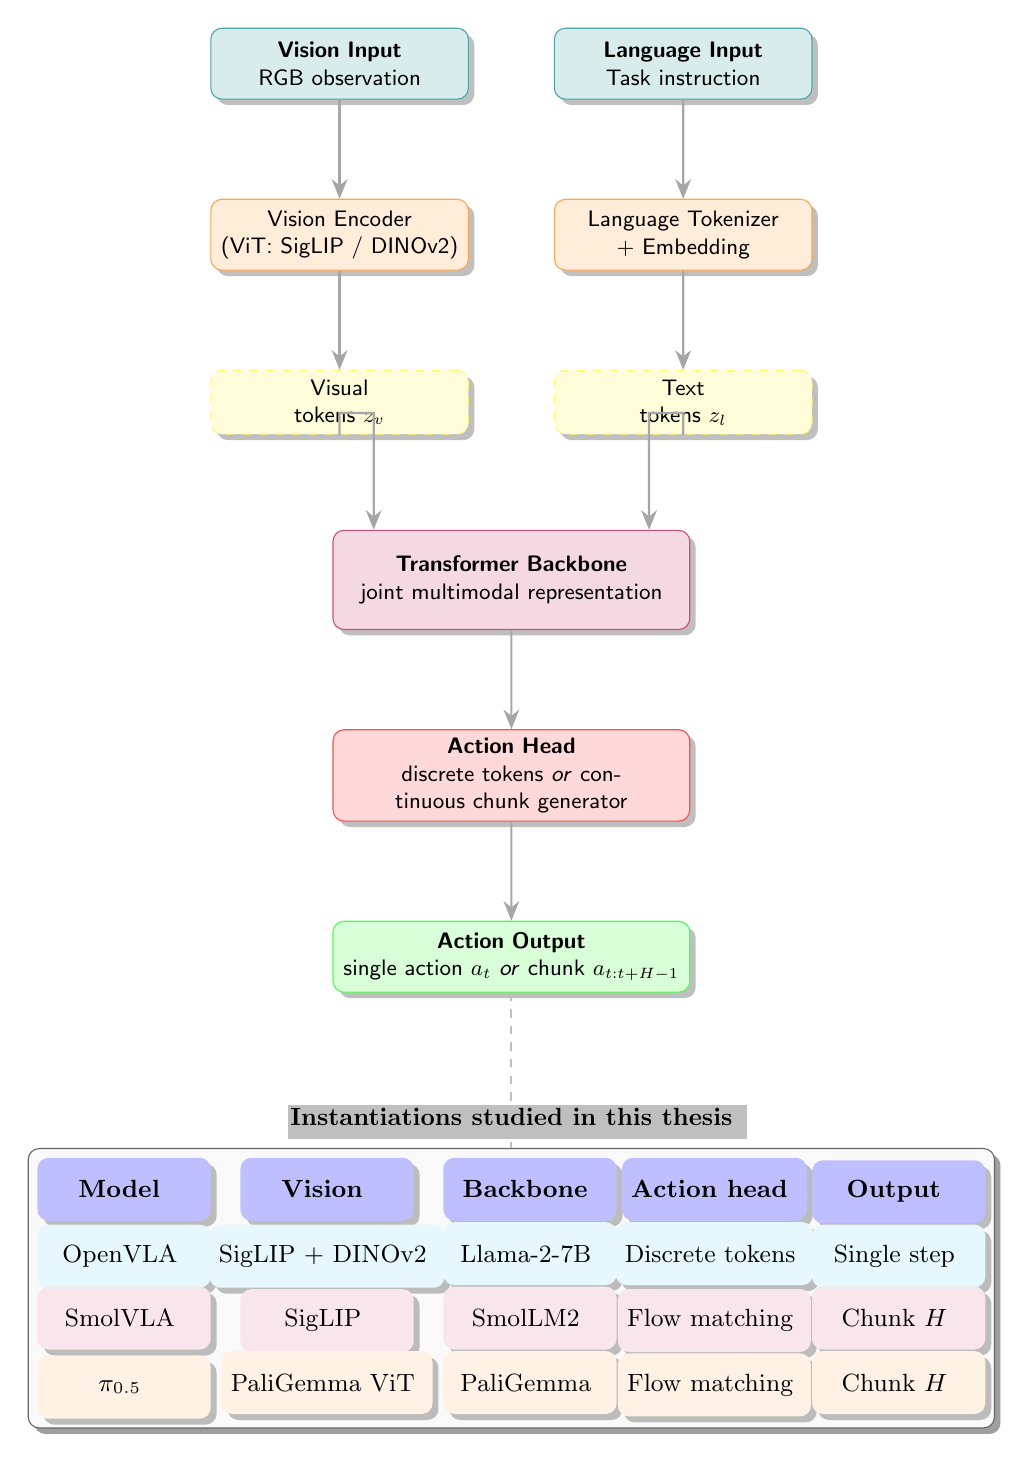
\begin{tikzpicture}[
  node distance=1.4cm and 1.2cm,
  scale=0.9,
  transform shape,
  every node/.style={align=center, font=\small\sffamily, drop shadow},
  input/.style={rectangle, rounded corners, draw=teal!70, fill=teal!15,
                text width=3.4cm, minimum height=1.0cm},
  encoder/.style={rectangle, rounded corners, draw=orange!70, fill=orange!15,
                  text width=3.4cm, minimum height=1.0cm},
  token/.style={rectangle, rounded corners, draw=yellow!60, fill=yellow!15,
                text width=3.4cm, minimum height=0.9cm, dashed},
  fusion/.style={rectangle, rounded corners, draw=purple!70, fill=purple!15,
                 text width=4.8cm, minimum height=1.4cm},
  head/.style={rectangle, rounded corners, draw=red!70, fill=red!15,
               text width=4.8cm, minimum height=1.2cm},
  output/.style={rectangle, rounded corners, draw=green!70, fill=green!15,
                 text width=4.8cm, minimum height=1.0cm},
  varheader/.style={fill=blue!25, font=\small\bfseries},
  arrow/.style={-{Stealth[length=2.5mm, width=2mm]}, thick, draw=gray!70}
]

% ---- Top: inputs ----
\node (vision) [input]                     {\textbf{Vision Input} \\ RGB observation};
\node (lang)   [input, right=of vision]    {\textbf{Language Input} \\ Task instruction};

% ---- Encoders ----
\node (venc)   [encoder, below=of vision]  {Vision Encoder \\ (ViT: SigLIP / DINOv2)};
\node (lenc)   [encoder, below=of lang]    {Language Tokenizer \\ + Embedding};

% ---- Tokens ----
\node (vtok)   [token, below=of venc]      {Visual \\ tokens $z_v$};
\node (ltok)   [token, below=of lenc]      {Text \\ tokens $z_l$};

% ---- Fusion ----
\coordinate (mid) at ($(vtok)!0.5!(ltok)$);
\node (fusion) [fusion, below=1.8cm of mid]
  {\textbf{Transformer Backbone} \\ joint multimodal representation};

% ---- Action Head ----
\node (head)   [head, below=of fusion]
  {\textbf{Action Head} \\ discrete tokens \emph{or} continuous chunk generator};

% ---- Output ----
\node (action) [output, below=of head]
  {\textbf{Action Output} \\ single action $a_t$ \emph{or} chunk $a_{t:t+H-1}$};

% ---- Arrows ----
\draw [arrow] (vision) -- (venc);
\draw [arrow] (lang)   -- (lenc);
\draw [arrow] (venc)   -- (vtok);
\draw [arrow] (lenc)   -- (ltok);
\draw [arrow] (vtok) -- ++(0,-0.15) -| (fusion.160);
\draw [arrow] (ltok) -- ++(0,-0.15) -| (fusion.20);
\draw [arrow] (fusion) -- (head);
\draw [arrow] (head)   -- (action);

% ---- Model Variants Table ----
\node (varlabel) [below=1.5cm of action, font=\bfseries]
  {Instantiations studied in this thesis};

\matrix (var) [
  below=0.2cm of varlabel,
  matrix of nodes,
  nodes={minimum height=0.8cm, minimum width=2.2cm, align=center, font=\small},
  column sep=-\pgflinewidth,
  row sep=-\pgflinewidth,
  draw=black!60,
  rounded corners,
  fill=gray!5,
  drop shadow
]
{
  |[varheader]| \textbf{Model} & |[varheader]| \textbf{Vision} &
  |[varheader]| \textbf{Backbone} & |[varheader]| \textbf{Action head} &
  |[varheader]| \textbf{Output} \\
  |[fill=cyan!10]| OpenVLA & |[fill=cyan!10]| SigLIP + DINOv2 &
  |[fill=cyan!10]| Llama-2-7B & |[fill=cyan!10]| Discrete tokens &
  |[fill=cyan!10]| Single step \\
  |[fill=purple!10]| SmolVLA & |[fill=purple!10]| SigLIP &
  |[fill=purple!10]| SmolLM2 & |[fill=purple!10]| Flow matching &
  |[fill=purple!10]| Chunk $H$ \\
  |[fill=orange!10]| $\pi_{0.5}$ & |[fill=orange!10]| PaliGemma ViT &
  |[fill=orange!10]| PaliGemma & |[fill=orange!10]| Flow matching &
  |[fill=orange!10]| Chunk $H$ \\
};

\draw [dashed, gray!50, thick] (action.south) -- ++(0,-0.5) -| (var.north);
\end{tikzpicture}
\caption{The common vision--language--action architecture and its instantiations. Visual and language inputs are separately encoded into token sequences, fused by a transformer backbone, and decoded by an action head. The table maps the three models studied in this thesis onto their component choices. The decisive distinction for this work is the final column: OpenVLA emits a single action per observation, whereas SmolVLA and $\pi_{0.5}$ emit an action chunk of horizon $H$.}
\label{fig:vla_general_with_variants}
\end{figure}



Despite differences in scale, backbone, and action representation, contemporary vision--language--action models share a common structural template: a visual encoder and a language encoder produce token sequences, a transformer backbone fuses them into a joint representation, and an action head maps that representation to robot commands. This section describes the workflow stage by stage, and presents the three models studied in this thesis---OpenVLA, SmolVLA, and $\pi_{0.5}$---as distinct solutions to it. 


% ===========================================================================
\subsubsection{Visual and Language input encoding}
\label{subsubsec:vision}

The vision stage requires two kinds of information that are in tension.
Manipulation requires geometric precision---where the target object and the end-effector are, and how they are oriented---while language conditioning requires semantic grounding, so that the token ``the red mug'' selects the correct region of the scene. Vision encoders pretrained for one of these objectives are not automatically good at the other, and the models studied here resolve the tension differently.

The common substrate is the Vision Transformer. An observation $I \in \mathbb{R}^{h_{\mathrm{im}} \times w_{\mathrm{im}} \times C}$, of height $h_{\mathrm{im}}$ and width $w_{\mathrm{im}}$, is divided into non-overlapping patches of size $P \times P$, which are flattened and linearly projected into a sequence of visual tokens $z_v \in \mathbb{R}^{M \times d}$ with $M = h_{\mathrm{im}}w_{\mathrm{im}}/P^2$. These tokens are projected by a small MLP into the backbone's embedding space so that they can be consumed alongside text tokens.

\paragraph{Visual encoders.}
Self-supervised encoders such as DINOv2~\cite{oquab2024dinov2learningrobustvisual} learn geometric information from images via self-distillation, in which a student network predicts the representations of an exponentially moving-average teacher, at both the image level (global--local view matching) and the patch level (masked patch prediction). Without language supervision, the features carry less categorical abstraction. Still, they provide sharper spatial segmentation and are robust to lighting and viewpoint variation---properties useful for localising small objects and the end-effector in a  workspace~\cite{karamcheti2024prismatic}.

\paragraph{Language encoders.}
Contrastive image--text pretraining yields encoders whose features align with language. SigLIP~\cite{zhai2023sigmoid} is the variant most commonly used in current VLAs. It replaces the batch-global softmax objective of CLIP \citep{radford2021learning} with a pairwise sigmoid loss, treating each image--text pair as an independent binary classification:
\begin{equation}
\mathcal{L}_{\mathrm{SigLIP}}
= -\frac{1}{B}\sum_{j=1}^{B}\sum_{k=1}^{B}
\log \sigma\!\left( y_{jk}\, z_{jk} \right),
\qquad
z_{jk} = e^{\sigma}(i_j \cdot t_k) + b,
\end{equation}
where $i_j$ and $t_k$ are image and text embeddings, $y_{jk} = +1$ for matched pairs and $-1$ otherwise, and $e^{\sigma}, b$ are a learned scale and bias. Decoupling the loss from batch-global normalisation removes a memory bottleneck and permits pretraining at very large scale. The resulting features excel at object identity and category, which is what language grounding requires.


\paragraph{Feature fusion.}
OpenVLA follows the Prismatic recipe~\cite{karamcheti2024prismatic} and uses both, fusing them by channel-wise concatenation of the per-patch feature vectors,
\begin{equation}
\tilde{z}_v^{(m)} =
\left[\, z_{v,\mathrm{sig}}^{(m)} \; ; \; z_{v,\mathrm{dino}}^{(m)} \,\right]
\in \mathbb{R}^{d_{\mathrm{sig}} + d_{\mathrm{dino}}}.
\end{equation}
Concatenating along the feature dimension rather than appending along the sequence dimension is deliberate: it preserves both signals in every token without doubling the sequence length, which would quadratically increase the attention cost in the backbone. SmolVLA, targeting efficiency, uses a single SigLIP-family encoder and accepts weaker geometric features in exchange for a smaller model. The $\pi$ family inherits the vision encoder of its PaliGemma-family VLM backbone, so the vision and language components are pretrained jointly rather than assembled from separately pretrained parts.

The language stage is the most uniform across models. The instruction is tokenized---typically by byte-pair encoding---and embedded into a sequence $z_l \in \mathbb{R}^{L \times d}$ of the same dimensionality as the projected visual tokens. Visual and text tokens are then concatenated into a single context sequence, \begin{equation}
X_{\mathrm{input}} = [\, z_l \; ; \; z_v \,],
\end{equation}
and passed through the transformer backbone, whose self-attention layers bind linguistic references to the visual regions they denote. Fusion is thus performed implicitly by the backbone rather than by a dedicated cross-modal module.

% ===========================================================================
\subsubsection{Backbone}
\label{subsubsec:language}
OpenVLA uses a Llama-2-7B decoder \citep{touvron2023llama}, a language model adapted post hoc to accept visual tokens. $\pi_{0.5}$ builds on a PaliGemma-family vision--language model, already multimodal before robot fine-tuning. SmolVLA uses a compact SmolLM-family backbone, trading capacity for trainability on modest hardware. The relevance to this thesis is indirect but real: backbone scale governs how quickly a model converges and how much data it needs, which is precisely what distinguishes the training regimes compared in Chapter~\ref{sec:results}.

% ===========================================================================
\subsubsection{Action output}
\label{subsubsec:action}

The action head is where the three models diverge most sharply, and where the divergence matters most for this thesis. Two questions define the design space: whether the action is represented discretely or continuously, and whether a forward pass emits one action or a chunk of $H$ consecutive actions. The
answers determine what a ``prediction'' is, and therefore what a validation metric can compare.

\paragraph{Discrete autoregressive actions.}
The first approach recasts control as token generation, so that the pretrained language backbone can be reused without architectural modification. Each dimension of the action is uniformly discretized into bins---$256$ in OpenVLA~\cite{kim2024openvla}, following RT-2~\cite{brohan2023rt2}---and the resulting indices are emitted autoregressively as tokens, then mapped back to continuous action values. For a $7$-DoF end-effector command the model produces seven tokens per timestep:
\begin{equation}
\mathbf{a}_t = (\Delta x, \Delta y, \Delta z,
\Delta\mathrm{roll}, \Delta\mathrm{pitch}, \Delta\mathrm{yaw}, g),
\end{equation}
with $g$ the binary gripper state. Training minimises a cross-entropy over these tokens.

The approach has three consequences. Discretization imposes a resolution floor, since no action finer than a bin can be expressed. Because tokens are sampled per dimension, correlations across dimensions are represented only weakly. And because one forward pass yields one action, the policy is Markovian with respect to the observation stream: temporal structure is not represented in the output at all. Thus, a single-step method can produce action trajectories with jerk and spikes.

\paragraph{Continuous chunk generation.}
The second approach attaches a generative head that emits a continuous action chunk directly, conditioned on the backbone's multimodal representation:
\begin{equation}
\pi_\theta(o_t) \;\mapsto\; (a_t, a_{t+1}, \dots, a_{t+H-1}).
\end{equation}
Flow matching~\cite{lipman2023flow} is the mechanism used by both SmolVLA~\cite{shukor2025smolvla} and the $\pi$ family~\cite{black2024pi0, intelligence2025pi05}: an ``action expert'' module integrates a learned velocity field from noise to the action sequence, conditioned on the observation representation, and is trained by regressing the velocity field along interpolation paths rather than by maximising a likelihood.

In contrast to the previous set, flow matching shows three properties. First, the action space is continuous, removing the resolution floor. Second, the chunk is generated jointly, so temporal correlations---smoothness, consistent direction of motion---are modeled explicitly in the output distribution rather than left to emerge across independent forward passes. Third, the natural unit of comparison against an expert demonstration is a trajectory segment rather than a single action, which makes geometric trajectory measures such as dynamic time warping and optimal transport applicable at all.

%% Yibo: does it make sense to replace NLL with this?
A fourth consequence bears on one candidate metric specifically. For discrete-token policies, a sequence likelihood is directly available and is essentially the training objective itself, so a negative-log-likelihood validation figure adds little information beyond the training loss. Flow-matching models admit no directly tractable likelihood; instead, an NLL for a flow-matching model refers to an approximation or bound obtained at additional computational cost. This thesis is therefore explicit about which model class each NLL result refers to.

\subsection{Categories of modern VLA architectures}
\label{sec:vla-categories}

Modern VLA models can be organised along several axes; the one that matters for trajectory-level validation is how the action is represented and emitted. This section adopts that axis.

\subsubsection{Autoregressive discrete-token policies}
\label{subsec:token-policies}

The first category treats action prediction as token generation. Each continuous action dimension is discretized into a fixed number of bins, and the resulting tokens are emitted autoregressively by the language-model backbone exactly as text tokens would be. RT-2~\cite{brohan2023rt2} established the approach and OpenVLA~\cite{kim2024openvla} is a widely used open instantiation.

The policy consumes one observation and produces one action $a_t$; obtaining the next action requires a new observation. Such a policy is effectively Markovian---a stateless function of the current observation, with no recurrent state carried across timesteps---and any historical information available to it is confined to what a single observation encodes.

Two properties follow. Because tokens are sampled per dimension, correlations across action dimensions and across time are represented only weakly. And because the objective is a cross-entropy over these tokens, the validation loss is a per-step teacher-forced quantity. 

\subsubsection{Continuous chunk-generating policies}
\label{subsec:chunk-policies}

The second category predicts a chunk of $H$ future actions from a single observation, in a continuous action space, using a generative head attached to the vision language backbone. Rather than sampling discrete tokens, these models denoise or integrate a whole action sequence jointly, so that temporal
correlations within the chunk---smoothness, consistent direction---are modeled directly in the output distribution.

Flow matching~\cite{lipman2023flow} has become the dominant mechanism in this category. The $\pi_0$ family~\cite{black2024pi0} couples a pretrained vision--language backbone with a flow-matching action expert producing high-frequency continuous action chunks, and $\pi_{0.5}$ \citep{intelligence2025pi05} extends this line with broader training for open-world generalisation. SmolVLA~\cite{shukor2025smolvla} pursues the same chunked, continuous formulation at a substantially smaller scale, targeting efficient training and deployment on accessible edge-computing hardware.

\subsection{VLA foundation models and evaluation benchmarks}
\label{sec:vla-foundation}

The models studied in this thesis extend behaviour cloning in two directions simultaneously: they condition on natural language, and they inherit representations from large-scale pretraining.

The motivation is generalisation. A policy trained by behaviour cloning on a fixed set of demonstrations typically transfers poorly to new objects, backgrounds, or phrasings of a task. Vision language models (VLM) pretrained on web-scale image--text corpora, by contrast, carry broad semantic and visual priors. Vision-language-action (VLA) models are built by taking such a pretrained backbone and fine-tuning it to output robot actions conditioned on an image observation and a language instruction, so that the semantic grounding of the backbone is transferred to control~\cite{brohan2023rt2}.

Despite the foundation-model framing, the learning pattern remains behaviour cloning: a supervised, teacher-forced, per-step objective over demonstrated actions, exactly as in Equation~\eqref{eq:bc}. The pretraining changes the representation and the generalisation, not the nature of the objective. The limitations identified in Section~\ref{subsec:bc-failure} therefore carry over intact, which is why a validation signal designed for behaviour cloning at the trajectory level remains necessary for VLA models.

Evaluating these models has correspondingly become a benchmark-driven activity. Standardised simulated suites such as LIBERO~\cite{liu2023libero} provide fixed task sets and demonstration data and report closed-loop success rate---the fraction of rollouts completing the task---as the headline measure. Success rate is the ground truth used throughout this thesis, and Section~\ref{sec:eval} discusses why it is nevertheless unsuitable as a training-time signal.


\subsection{Training and Fine-tuning}
\label{sec:vla-training}

Vision language action (VLA) models acquire a joint distribution over observations and actions through large-scale pretraining on heterogeneous robot data, such as the Open X-Embodiment (OXE) collection, which aggregates demonstrations spanning many robot embodiments, tasks, and environments. OpenVLA instantiates this paradigm by coupling a fused DINOv2--SigLIP visual encoder with a Llama~2 7B language backbone---the latter pretrained on approximately two trillion text tokens---and training the resulting policy on roughly $970\text{k}$ real-world manipulation trajectories drawn from OXE~\cite{kim2024openvla}. Continuous actions are represented as discrete tokens by uniformly binning each action dimension into $256$ intervals and mapping them onto reserved entries of the language model vocabulary, so that closed-loop control reduces to next-token prediction. Through this pretraining, the model attains a broadly generalizable control policy capable
of zero-shot execution across previously unseen objects, scenes, and instructions.

When confronted with a new embodiment, an unfamiliar task, or an out-of-distribution environment, however, a pretrained VLA may lack the task-specific structure required for reliable control, and its zero-shot
performance degrades accordingly. Fine-tuning addresses this gap by continuing to update the model weights on a task-specific dataset, aligning the policy with the target distribution and improving inference
performance~\cite{kim2024openvla}.

The benefits of fine-tuning are threefold. First, it is computationally economical: reusing pretrained weights removes the need for training from scratch and substantially reduces GPU time. Second, it rapidly improves task-specific accuracy by adapting the learned representation to the target objects, dynamics, and
objectives, while keeping the general understanding of the world. Third, when combined with parameter-efficient fine-tuning (PEFT), it remains effective under limited data and hardware budgets, since only a small fraction of the parameters is updated. The remainder of this section develops the PEFT scheme adopted here, low-rank adaptation, and the optimizer that drives it.

\subsubsection{Low-Rank Adaptation}
\label{sec:lora}

Low-rank adaptation (LoRA) is a parameter-efficient fine-tuning method for large language models~\cite{hu2021loralowrankadaptationlarge}. Neural networks are built largely from dense, full-rank weight matrices, and adapting a pretrained weight $W_0 \in \mathbb{R}^{d\times k}$ to a new distribution can be written as $W = W_0 + \Delta W$. Because updating all parameters of a multi-billion-parameter
model is both costly and, empirically, unnecessary---task adaptation has been shown to possess a low intrinsic dimension~\cite{aghajanyan2020intrinsicdimensionalityexplainseffectiveness}---LoRA constrains the update to a low rank $r \ll \min(d,k)$ and factorizes it as $\Delta W = BA$, with $B \in \mathbb{R}^{d\times r}$ and $A \in \mathbb{R}^{r\times k}$. A layer's forward pass then becomes
\begin{equation}
h = Wx = W_0 x + \frac{\alpha}{r}\, B A x,
\label{eq:lora-forward}
\end{equation}
where $\alpha$ is a scaling hyperparameter that controls the magnitude of the adaptation relative to the frozen backbone. During fine-tuning $W_0$ is frozen and only $A$ and $B$ are optimized, which reduces the number of trainable parameters by orders of magnitude and shrinks the storage required per task to the incremental factors alone.

To start fine-tuning from the exact pretrained state and to preserve stability, the factors are initialized asymmetrically,
\begin{equation}
A \sim \mathcal{N}(0, \sigma^2), \qquad B = \mathbf{0},
\label{eq:lora-init}
\end{equation}
so that $\Delta W = \mathbf{0}$ at the first iteration and the pretrained representation is left intact; a nonzero initialization would instead perturb the weights immediately, which can destabilize training in large models whose representations are sensitive to such shifts. This asymmetry also shapes the first
gradients. With $B = \mathbf{0}$, the gradient with respect to $A$ vanishes,
\begin{equation}
\frac{\partial \mathcal{L}}{\partial A}
= B^{\top} \frac{\partial \mathcal{L}}{\partial \Delta W} = \mathbf{0},
\end{equation}
whereas the gradient with respect to $B$ does not,
\begin{equation}
\frac{\partial \mathcal{L}}{\partial B}
= \frac{\partial \mathcal{L}}{\partial \Delta W} A^{\top} \neq \mathbf{0}.
\end{equation}
Consequently the first optimization step updates $B$ alone; once $B$ departs from zero, $A$ begins to adapt as well, so that the model moves smoothly away from the pretrained solution rather than jumping abruptly.

\subsubsection{Optimization}
\label{sec:optimization}

Under the low-rank parameterization, fine-tuning reduces to optimizing only the factors $A$ and $B$ while the backbone $W_0$ remains frozen. Collecting the trainable parameters as $\boldsymbol{\theta} = \{A, B\}$ ($\approx\!80\text{M}$ at rank $r = 32$), the objective minimizes the per-token cross-entropy of the discretized action tokens over the task dataset $\mathcal{D}$:
\begin{equation}
\boldsymbol{\theta}^\star
= \arg\min_{\boldsymbol{\theta}}\;
\mathbb{E}_{(x,a)\sim\mathcal{D}}
\left[
-\sum_{k} \log p_{\,W_0 + \Delta W(\boldsymbol{\theta})}\!\left(a_k \mid a_{<k},\, x\right)
\right].
\label{eq:objective}
\end{equation}
Because $\boldsymbol{\theta}$ comprises heterogeneous matrices injected across the attention and MLP projections, whose gradients differ by orders of magnitude between layers, an adaptive per-parameter optimizer is preferable to plain stochastic gradient descent, for which a single global learning rate cannot suit all coordinates at once. The optimizer used throughout is AdamW~\cite{loshchilov2017decoupled}, the decoupled-weight-decay variant of Adam~\cite{kingma2014adam}.

Let $g_t = \nabla_{\boldsymbol{\theta}} \Loss_t(\boldsymbol{\theta}_{t-1})$ denote the stochastic gradient at step $t$. Adam maintains two exponential moving averages of the gradient and applies a bias correction that compensates for their zero initialization.
\begin{align}
m_t &= \beta_1 m_{t-1} + (1-\beta_1)\, g_t
      \label{eq:adam-m}\\
v_t &= \beta_2 v_{t-1} + (1-\beta_2)\, g_t^{2}
      \label{eq:adam-v}\\
\mhat_t &= \frac{m_t}{1-\beta_1^{\,t}}, \qquad
\vhat_t = \frac{v_t}{1-\beta_2^{\,t}}
      \label{eq:adam-bias}\\
\boldsymbol{\theta}_t &= \boldsymbol{\theta}_{t-1}
      - \eta\, \frac{\mhat_t}{\sqrt{\vhat_t}+\epsilon},
      && \label{eq:adam-update}
\end{align}
with defaults $\beta_1 = 0.9$, $\beta_2 = 0.999$, and $\epsilon = 10^{-8}$. The factor $\eta / (\sqrt{\vhat_t}+\epsilon)$ acts as an effective per-parameter learning rate: coordinates with large, noisy gradients take smaller steps, while stable ones take larger steps, which is precisely what the scale heterogeneity of the adapter weights demands. AdamW further decouples weight decay from the gradient, applying it directly to the weights rather than through the moment estimates,
\begin{equation}
\boldsymbol{\theta}_t = \boldsymbol{\theta}_{t-1}
- \eta\left(\frac{\mhat_t}{\sqrt{\vhat_t}+\epsilon}
+ \lambda\, \boldsymbol{\theta}_{t-1}\right),
\label{eq:adamw-update}
\end{equation}
which is preferable to Adam with $L_2$ regularization, where the penalty folded into $g_t$ is subsequently rescaled by $\sqrt{\vhat_t}$ and thereby coupled to gradient magnitude.

The moments $(m_t, v_t)$, together with the step counter $t$, constitute the optimizer state: one value each per trainable parameter. This state is distinct from the model weights---whereas $\boldsymbol{\theta}$ encodes where the model is, $(m,v)$ encode how it has been moving to get there---and two of its properties bear on the experiments that follow. First, its memory footprint scales with the number of trainable parameters: for $P$ parameters in single precision the state occupies $8P$ bytes ($\sim\!0.6\,\text{GB}$ here, as opposed to the $\sim\!56\,\text{GB}$ that training the full $7\text{B}$ backbone would demand), which reinforces the efficiency argument for PEFT. Second, because $(m,v)$ are moving averages of the entire gradient history, they are path-dependent and cannot be reconstructed from the final weights; to be recoverable, they have to be checkpointed explicitly.

The step actually taken is $\eta$ times the adaptive direction, so the learning-rate schedule $\eta(t)$ governs stability. A constant rate $\eta = 5\times 10^{-4}$ is used. When the second moment $\vhat_t$ is a poor estimate---at the very start of training, or immediately after the optimizer state is reset---the adaptive denominator in Eq.~\eqref{eq:adam-update} is unreliable and the resulting steps are poorly calibrated; a warmup schedule $\eta(t) = \eta_{\max}\, t / T_w$, which ramps the rate over $T_w$ steps, keeps the early updates bounded while $(m,v)$ stabilize. This consideration is central to the continual fine-tuning experiments of Section~\ref{sec:exp-continual}.

\subsection{Robotics End-Effector Pose Representation}
\label{sec:pose-representation}
The robot arm is controlled by seven joint angles: one joint controls the gripper's opening and closing, and six sequential joints control the arm's pose. Together these determine the end-effector's pose relative to the main body, so how that pose is represented has a direct effect on downstream control and learning.

\subsubsection{Coordinate Frames}

In robotic manipulation, the coordinate frames represent the perspective to describe the position and orientation of robot components and objects in the 3D space. A frame is typically defined as a right-handed coordinate system consisting of an origin and three orthogonal axes. In robots like Spot, multiple frames coexist, typically including: 
\begin{itemize}
    \item \textbf{odometry frame}, the origin is fixed to the starting position and orientation of the robot's tail point. It is a global frame, which does not move with the robot. The frame may drift over time due to accumulated sensor noise or errors.
    \item \textbf{body frame}, the origin moves with the position and orientation of the robot's tail. It is a local frame. The end-effector pose with respect to the body is intuitive in the body frame. 
    \item \textbf{flat body frame}, the origin moves with the position of the robot's tail, while the Z-axis points upwards, aligning with the gravity direction. It is convenient for stabilizing the orientation when the quadruped robot twists its body or walks onto uneven terrain. 
    \item \textbf{camera frame}, attached to the robot's camera. The origin is at the camera's optical center or the upper-left corner, used for object localization in computer vision tasks.
\end{itemize}

Transformations between frames enable consistent representation of kinematic relationships across different parts of the robot and environment, which are critical for accurate motion execution and manipulation tasks.
Rigid body transformations are commonly represented using homogeneous transformation matrices in SE(3), represented as:

\begin{equation}
\mathbf{T} =
\begin{bmatrix}
\mathbf{R} & \mathbf{t} \\
0 & 1
\end{bmatrix} \in \mathrm{SE}(3)
\end{equation}

where $\mathbf{R}\in \mathrm{SO}(3)$ represents rotation and $\mathbf{t}\in \mathbb{R}^3$ represents translation. 


\subsubsection{Rotation Representation}
Euler angles and quaternions are the two primary ways to represent 3D rotations in robotics. 

\textbf{Euler angle} is a classical method for representing 3-dimensional orientations using three sequential rotations about specific coordinate axes. Among the six possible sequences of three distinct axes, ZYX is the most common rotation sequence, shown as Figure \ref{fig:spot_euler}, where
 \textit{roll} angle $(\phi)$ is  the rotation about the $x$-axis; \textit{pitch} angle $(\theta)$ the rotation about the $y$-axis; \textit{yaw} angle $(\psi)$ is the rotation about the $z$-axis. 

\begin{figure}[htb]
    \centering 
    \includegraphics[height=8cm]{Spot_eura_angle.png}
    \caption{The Euler angles of the Spot robot~\cite{spot_euler}.}
    \label{fig:spot_euler}
\end{figure}

The robot arm is modeled as a 7-DoF serial manipulator, whose end-effector pose is uniquely determined by Forward Kinematics (FK)~\cite{fk} in the task space as $$\mathbf{x} = [x, y, z, \phi, \theta, \psi, g]^T,$$ where $(x, y, z) \in \mathbb{R}^3$ is the positional component in Cartesian coordinates, and $(\phi, \theta, \psi) \in \mathbb{R}^3$ are the orientation components represented as Euler angles in the ZYX rotation sequence, $g$ is a bool variable representing the open and close state of the gripper. 

\begin{figure}[!htb]
    \centering
    \includegraphics[height=8cm]{spot_arm_joint.png}
    \caption{Spot Arm joint designations, range of motion, and length of links (in millimeters)~\cite{spot_arm}}
    \label{fig:arm_joint}
\end{figure}
The Euler angle is intuitive for visualization and human manipulation. However, this representation suffers from several classic drawbacks such as gimbal lock and interpolation.~\cite{robotics}. 


\textbf{Quaternion} offers an alternative representation that avoids many of the issues associated with Euler angles~\cite{quat}. A unit quaternion is a four-dimensional vector \(\mathbf{q} = (q_w, q_x, q_y, q_z) \in \mathbb{R}^4\) constrained to lie on the unit three-dimensional sphere, i.e., \(\|\mathbf{q}\| = 1\), calculated by:

$$q_w=\mathrm{cos}(\frac{\psi}{2})\mathrm{cos}(\frac{\theta}{2})\mathrm{cos}(\frac{\phi}{2})+\mathrm{sin}(\frac{\psi}{2})\mathrm{sin}(\frac{\theta}{2})\mathrm{sin}(\frac{\phi}{2})$$
$$q_x=\mathrm{cos}(\frac{\psi}{2})\mathrm{sin}(\frac{\theta}{2})\mathrm{cos}(\frac{\phi}{2})-\mathrm{sin}(\frac{\psi}{2})\mathrm{cos}(\frac{\theta}{2})\mathrm{sin}(\frac{\phi}{2})$$
$$q_y=\mathrm{cos}(\frac{\psi}{2})\mathrm{cos}(\frac{\theta}{2})\mathrm{sin}(\frac{\phi}{2})+\mathrm{sin}(\frac{\psi}{2})\mathrm{sin}(\frac{\theta}{2})\mathrm{cos}(\frac{\phi}{2})$$
$$q_z=\mathrm{sin}(\frac{\psi}{2})\mathrm{cos}(\frac{\theta}{2})\mathrm{cos}(\frac{\phi}{2})-\mathrm{cos}(\frac{\psi}{2})\mathrm{sin}(\frac{\theta}{2})\mathrm{sin}(\frac{\phi}{2})$$

A quaternion represents a 3D rotation by defining a single rotation of angle $\alpha$ around a fixed axis unit vector $\mathbf{u}=(u_x, u_y, u_z)$, 

$$\mathbf{q}=\left(\cos\frac{\alpha}2\;,\mathbf{u}\sin\frac\alpha2\;\right)=\left(\cos\frac\alpha2\;,u_{x}\sin\frac\alpha2\;,u_{y}\sin\frac\alpha2\;,u_{z}\sin\frac\alpha2\;\right)$$

Unlike Euler angles, which describe a sequence of rotations, this "axis-angle" pair $(\alpha, \mathbf{u})$ describes the transformation in one step.

Mathematically, a quaternion $\mathbf{q}$ is an extension of complex numbers, written as:
$$\mathbf{q}=w+x\mathbf{i}+y\mathbf{j}+z\mathbf{k}$$

This representation is free of gimbal lock and singularities, also supports continuous interpolation and differentiation, making it particularly suitable for robotic control applications, offering the following advantages where Euler angles fail~\cite{robotics}.
 
First, avoiding gimbal lock: In robotic arm control, gimbal lock is the loss of one rotational degree of freedom that occurs when two rotational axes become parallel, most commonly when the pitch angle reaches ±90°, causing the remaining roll and yaw motions to produce identical effects and rendering the arm unable to move freely in that direction. While Euler angles inherently suffer from this singularity due to their sequential, fixed-axis rotations, quaternions do not, as they encode a single orientation as a rotation about an arbitrary axis without relying on dependent steps. The most robust solution is to use quaternions internally for all computations and trajectory interpolation, converting to Euler angles only for human-readable displays; additional practical measures include switching to tool-coordinate control, employing rotation matrices, or introducing redundant degrees of freedom (e.g., 7-axis arms) to handle kinematic singularities through task-priority algorithms.

Second, smooth interpolation. The mapping from rotation matrices to Euler angles is not continuous throughout the entire space of rotations, leading to instability during interpolation and differentiation. These characteristics make Euler angles problematic for continuous orientation control, especially in extreme cases of robotic systems. Quaternions allow for Spherical Linear Interpolation (SLERP), which finds the shortest, most natural path between two orientations.

$$S L E R P(q_{0},q_{1};t)={\frac{\sin((1-t)\Omega)}{\sin\Omega}}\;q_{0}+{\frac{\sin(t\Omega)}{\sin\Omega}}\;q_{1}$$

\textbf{Mapping between Euler angles and quaternions} is not strictly unique. Converting Euler angles to a quaternion is unique, but the reverse mapping is not, due to the 360° angular periodicity and gimbal-lock singularities where infinite roll-yaw pairs collapse into the same quaternion. To produce a deterministic, one-to-one output, most robotics libraries enforce common range constraints—typically restricting pitch to [-90°, 90°) and roll/yaw to [-180°, 180°) to extract a canonical set of angles. However, even with these bounds, a true bijection does not exist at the singularities, where the solution remains degenerate.



\clearpage

\section{Problem: early stopping and evaluation criteria for VLA models}
\label{sec:eval}

Early stopping is a regularization technique that halts training when performance on a validation set begins to degrade. Even if training loss keeps improving, the validation performance eventually worsens due to overfitting. Early stopping tries to capture the turning point when the validation metric does not improve within a tolerated number of epochs. This approach is widely used because it is simple while effectively ensuring the model's generalization performance. 

\subsection{The evaluation gap}
\label{subsec:eval-gap}

Two quantities are available to a practitioner training a VLA policy, and neither is satisfactory as a training-time selection signal.

Closed-loop success rate is the measure that matters, but obtaining it requires executing many rollouts per checkpoint in simulation or on hardware. It is expensive, high-variance when the number of episodes is small, and available only after the fact---properties that make it impractical as a signal for early
stopping during training.

Offline validation loss is cheap and available at every evaluation step, but is structurally misaligned with trajectory quality. Three arguments establish this, and together they constitute the necessity argument of the thesis.

\paragraph{It is a teacher-forced per-step surrogate.}
As set out in Sections~\ref{subsec:bc-failure} and~\ref{subsec:token-policies}, the loss---cross-entropy over action tokens, or a flow-matching regression loss on noised targets---is computed conditioned on ground-truth context and averaged over independently treated timesteps. It never evaluates a rolled-out trajectory in which the model's own actions determine subsequent states, and is therefore blind to compounding error.

\paragraph{It is not aligned with task success.}
In behaviour cloning, it is repeatedly observed that validation loss correlates only weakly with closed-loop success, and that the loss-minimising checkpoint is not guaranteed to be the success-maximising one. Early stopping on validation loss may therefore select a checkpoint that is suboptimal in the only sense that matters at deployment. This thesis quantifies that cost directly as selection regret: the success-rate gap between the checkpoint a signal selects and the true best checkpoint.

\paragraph{Averaging conceals structure.}
Because the loss is a scalar mean of per-step errors, two action sequences with identical mean error can differ qualitatively---one smooth but lagged, the other correctly timed but jittery---while remaining indistinguishable to the objective. It cannot separate errors of shape from errors of phase.

\subsubsection{Trajectory comparison measures as offline validation signals}
\label{subsec:metrics}

The measures evaluated in this thesis compare a predicted action trajectory against a reference expert trajectory. Each captures a different notion of similarity, and each carries a characteristic failure mode; formal definitions appear in Chapter~\ref{sec:method}.

\paragraph{Per-step distances.}
The $L_1$ and $L_2$ distances between predicted and reference actions are the trajectory-space analogues of the training loss and serve as baselines against which the geometric measures are judged. They inherit the averaging limitation above.

\paragraph{Cosine distance.}
Cosine distance compares the direction of action vectors and is scale-invariant and inexpensive, but is by construction blind to action magnitude and, averaged per step, captures no more sequence-level structure than a per-step distance.

\paragraph{Dynamic time warping.}
DTW~\cite{sakoe1978dtw, muller2007information} measures similarity under an optimal temporal alignment and is therefore tolerant of phase lag and speed differences that per-step distances penalise heavily. That tolerance is also its weakness: by warping the time axis it discards timing information, so a correctly shaped trajectory executed at the wrong speed may score well. It is not a proper metric---the triangle inequality fails---and its cost is quadratic in sequence length; constrained and differentiable variants
\citep{cuturi2017soft} address part of this.

\paragraph{Optimal-transport distances.}
Wasserstein distances~\cite{villani2009optimal, peyre2019computational} treat trajectories, or the distributions of their waypoints, as distributions of mass and measure the minimal transport cost between them. They are geometry-aware and, unlike DTW, define a true metric. Applied naively to an unordered set of
waypoints, however, they discard temporal ordering unless it is reintroduced---by appending a time coordinate, or through a temporally regularised formulation---so it should be stated explicitly whether a trajectory is compared as an ordered curve or as a point cloud.

\paragraph{Negative log-likelihood.}
NLL is the only explicitly probabilistic candidate, scoring the reference
trajectory under the policy's predictive distribution and thereby reflecting
calibration rather than point error alone. 

\subsection{Relation to offline policy selection}
\label{subsec:ops}

Choosing a checkpoint without recourse to closed-loop rollouts is an instance of offline policy selection: ranking candidate policies using only offline data. The problem has been studied chiefly within offline reinforcement learning and off-policy evaluation, where estimators of expected return are used to rank
policies and are themselves benchmarked for ranking fidelity \citep{paine2020hyperparameter, fu2021benchmarks}.

By measuring trajectory-geometry metrics as offline policy-selection signals and comparing them
against closed-loop success as the ground truth, judged by both selection regret and rank
correlation, the effectiveness of the offline validation signals can be verified, so that the
earliest sufficiently good policy can be chosen on that basis.

The approach of choosing a policy is motivated by two properties. First, the candidate policies are imitation-learned VLAs whose quality is naturally assessed by geometric agreement with expert demonstrations rather than by reward estimation, which makes trajectory comparison measures a more
direct instrument than value-based estimators. Second, the practical problem is not to rank arbitrary policies but to select among checkpoints along a single training run, where candidates are strongly ordered by training progress, and the purpose is focused on early stopping alone.

\section{Method}
\label{sec:method}

\subsection{Overview}
\label{sec:method-overview}

This thesis proposes a lightweight offline substitute for closed-loop checkpoint evaluation, applied identically to every checkpoint a fine-tuning run produces. The method has three parts. First, each checkpoint's action prediction on held-out expert data is scored by one of several trajectory-comparison metrics: distances that treat the predicted and expert action chunks as sequences to be aligned or as distributions to be matched, together with an architecture-appropriate likelihood or loss surrogate (\S\ref{sec:method-metrics}). Second, the resulting per-checkpoint score is passed through a single early-stopping rule that reduces a whole metric curve to one selected checkpoint, so that every candidate metric is turned into a decision on equal footing (\S\ref{sec:method-selection}). Third, since an offline metric is only useful insofar as it stands in for an expensive online rollout, the method also fixes how to judge it: a candidate metric's ranking of checkpoints, and the single checkpoint it selects, are scored against the true closed-loop success curve by rank correlation and by the success forgone relative to the best checkpoint that was actually available (\S\ref{sec:method-eval}). \S\ref{sec:method-notation} below first fixes the notation these three parts share.

\subsection{Problem Statement and Notation}
\label{sec:method-notation}

Fine-tuning a VLA policy produces a sequence of checkpoints $\theta_0,\theta_1,\dots,\theta_K$, each inducing a policy $\pi_k=\pi_{\theta_k}$. Selecting which checkpoint to deploy is an early-stopping problem: the only trustworthy signal of deployment quality is closed-loop task success $Q(k)$, but measuring $Q(k)$ for every checkpoint requires either a real robot or a costly simulator rollout, which is exactly what the method above is designed to avoid needing at every step.
Here write $A^\star=(a^\star_0,\dots,a^\star_{H-1})$ for an expert action chunk of horizon $H$ drawn from
a held-out validation trajectory, and $A_k$ for the corresponding chunk produced by checkpoint $k$. For
a one-step (token-autoregressive) policy such as OpenVLA, $A_k$ is formed by teacher forcing: the
policy is queried at every expert state $h^\star_{t+j}$ along the window, $a_{k,j}=\pi_k(\,\cdot\mid
h^\star_{t+j})$. For a chunking policy such as SmolVLA or $\pi_{0.5}$, $A_k=\pi_k(\cdot\mid h^\star_t)$
is produced natively as a single forward pass. Both settings measure open-loop action quality on expert
inputs.

\subsection{Offline Validation Metrics}
\label{sec:method-metrics}

Four metrics are considered, all normalized so that lower is better. Actions are
standardized per dimension using training-split statistics before any distance is computed,
$\bar a_d=(a_d-\mu_d)/(\sigma_d+\epsilon)$, so that translation, rotation, and gripper channels
contribute comparably.

\paragraph{Dynamic Time Warping (DTW).} DTW admits nonlinear temporal alignment between two sequences,
which is appropriate when the same underlying behavior may be executed at a slightly different pace
\cite{sakoe1978dtw}. With pointwise cost $c(u,v)=\lVert u-v\rVert_2^2$ and $\Gamma$ ranging over
monotone warping paths,
\begin{equation}
  D_{\mathrm{DTW}}(X,Y) = \frac{1}{|\Gamma^\star|}\min_{\Gamma}\sum_{(r,u)\in\Gamma} c(x_r,y_u).
  \label{eq:dtw}
\end{equation}

\paragraph{Optimal Transport (OT).} Where DTW enforces a single monotone correspondence, entropic OT
compares the two sequences as empirical distributions over their elements, admitting soft many-to-many
correspondence \cite{cuturi2013sinkhorn}. With $p,q$ uniform over the sequence elements and $\Pi(p,q)$
the transport polytope,
\begin{equation}
  D^{\varepsilon}_{\mathrm{OT}}(X,Y) = \min_{\Gamma\in\Pi(p,q)} \sum_{r,u}\Gamma_{ru}\,c(x_r,y_u)
    + \varepsilon\sum_{r,u}\Gamma_{ru}\big(\log\Gamma_{ru}-1\big).
  \label{eq:ot}
\end{equation}

\paragraph{Cosine distance.} Cosine distance discards magnitude and measures only directional
agreement per timestep,
\begin{equation}
  D_{\cos}(X,Y) = 1-\frac{1}{H}\sum_{j=0}^{H-1}\frac{x_j^\top y_j}{\lVert x_j\rVert_2\lVert y_j\rVert_2+\epsilon}.
  \label{eq:cos}
\end{equation}
Because it is magnitude-blind, it is used only in conjunction with, never in place of, the metrics above.

\paragraph{Likelihood and architecture-specific surrogates.} The methodologically correct quantity is
the log-likelihood the policy assigns to the expert action under the expert state,
$\log\pi_k(a^\star_t\mid h^\star_t)$, not the likelihood of the policy's own rollout (an overconfident
but wrong policy can assign high likelihood to its own errors). Not every architecture exposes a
tractable likelihood, so the correct surrogate is architecture-dependent: token negative log-likelihood
for a discrete-token policy, $L_1$/$L_2$ validation error for a deterministic continuous policy, and the
validation flow-matching (or diffusion) objective for a flow-matching policy. This distinction matters:
OpenVLA's NLL is a genuine token log-likelihood,
whereas SmolVLA's and $\pi_{0.5}$'s ``NLL'' is the flow-matching validation loss standing in for one,
reported under the same key so the two are visually comparable but are not the same statistical object.

\subsection{Early-Stopping Selection Rule}
\label{sec:method-selection}

Given a checkpoint-level score $\bar m(k)$, the induced early-stopping rule selects the earliest checkpoint within a small tolerance of the metric's best observed value, rather than the checkpoint that literally minimizes $\bar m$ (which would overfit to a single noisy point):
\begin{equation}
  k_m^\star = \min\Big\{k : \bar m(k) \le \min_j \bar m(j) + \eta_m\Big\}, \qquad
  \eta_m = 0.01\,\big|\bar m(0)-\min_j \bar m(j)\big|.
  \label{eq:selection}
\end{equation}
For a metric that is higher-is-better (token accuracy is the only such case in this study) the inequality and the arguments to $\min$/$\max$ in Eq.~\ref{eq:selection} are reversed.

\subsection{Evaluating a Metric: Rank Correlation and Selection Regret}
\label{sec:method-eval}

A candidate metric $m$ is judged against the closed-loop success curve $Q(k)$ by two complementary statistics, computed only over the checkpoints at which both $\bar m(k)$ and $Q(k)$ are available:
\begin{equation}
  \rho_m = \mathrm{Spearman}\big(-\bar m(k),\,Q(k)\big),
  \qquad
  \mathrm{Regret}(m) = \max_k Q(k) - Q\big(k_m^\star\big).
  \label{eq:rho-regret}
\end{equation}
Spearman's rank correlation \cite{spearman1904} is preferred to a parametric correlation because the relationship between a validation distance and a bounded success rate is monotone but not linear.
$\rho_m$ near $+1$ indicates that the metric ranks checkpoints in the same order as closed-loop success; $\mathrm{Regret}(m)$ is the success forgone, in absolute percentage points, by trusting the metric's selection $k_m^\star$ instead of the checkpoint that was in fact best. A good metric has a high $\rho_m$ and low regret; the two need not agree in every instance, since regret depends on where $Q$ happens to be noisy near $k_m^\star$, while $\rho_m$ aggregates over the whole curve.

\section{Research Questions}
\label{sec:rq}

The evaluation gap of \S\ref{subsec:eval-gap} and the method formalized in \S\ref{sec:method} motivate a single practical question: which offline validation metric, computed cheaply from held-out demonstrations at every checkpoint, best predicts the closed-loop success rate that would otherwise require a costly rollout to observe? Answering it responsibly requires answering four narrower questions first, each a precondition or a robustness check on the one before it, plus a fifth that asks whether the same substitution extends from the checkpoint to a deployment-time hyperparameter. \S\ref{sec:implementation} describes how each is designed and implemented, and \S\ref{sec:results} reports the outcome of each, in the same order.

\subsection{RQ1: Do the candidate metrics carry any information about action quality at all?}
\label{sec:rq1}

Before a distance between a predicted and a reference trajectory can be trusted as a proxy for closed-loop success, it must first be shown to be informative about task identity on ground-truth data alone, independent of any policy. If a metric cannot separate two demonstrations of the same LIBERO-Goal task from a demonstration of a different task, it carries no task information and cannot measure action quality at all --- it is disqualified before RQ2 is even asked. This is a necessary, model-independent precondition, verified in \S\ref{sec:method-taskdisc} and \S\ref{sec:results-taskdisc}.

\subsection{RQ2: Do the offline metrics correlate with closed-loop task success, across architectures and training-set sizes?}
\label{sec:rq2}

This is the thesis's central question, and the one that verifies the practical effectiveness of the proposed metrics: whether a cheap, checkpoint-wise offline signal predicts the online success rate $Q(k)$ well enough to substitute for it. It is tested identically across three architectures --- discrete-token and flow-matching --- and two training-set sizes, so that any observed correlation cannot be dismissed as an artifact of one model family or one amount of data. Designed in \S\ref{sec:design-rq2}; answered in \S\ref{sec:results-crossmodel}--\S\ref{sec:results-permodel}.

\subsection{RQ3: Is metric-based early stopping actually effective in practice?}
\label{sec:rq3}

A correlation computed over an entire training run conflates an easy regime (leaving initialization, where both the metric and success move quickly) with a hard one (fine-ranking checkpoints that have already converged). A metric is only useful for early stopping if it also degrades gracefully, rather than catastrophically, once training reaches that harder regime. This question further asks whether any of the five runs --- three of them deliberately designed to induce it --- exhibits genuine action-quality overtraining, since a metric's value as an early-stopping signal is most directly demonstrated by its ability to catch a real decline rather than merely to track improvement. Designed in \S\ref{sec:method-plateau}; answered in \S\ref{sec:results-plateau}.

\subsection{RQ4: Which apparent differences between metrics, and between architectures, are statistically defensible?}
\label{sec:rq4}

Every $\rho_m$ reported for RQ2--RQ3 is a point estimate computed from as few as $11$ simulator evaluations. This question asks how much of any apparent ranking between two metrics, or any apparent split between architectures, survives resampling --- so that the conclusions of \S\ref{sec:results-conclusions} distinguish a genuine effect from sampling noise rather than over-reading a point estimate. Designed in \S\ref{sec:method-bootstrap}; answered in \S\ref{sec:results-bootstrap}.

\subsection{RQ5: Can an offline metric select the replan horizon, not only the checkpoint?}
\label{sec:rq5}

RQ1--RQ4 fix $h$, the open-loop action horizon (\texttt{n\_action\_steps}, i.e.\ how many actions of a predicted chunk a chunking policy executes before re-observing and re-planning), and let $\bar m(k)$ vary with the checkpoint $k$. This question inverts that: with a checkpoint fixed, does an offline metric's minimum over $h$ coincide with closed-loop success's maximum over $h$? It matters independently of RQ1--RQ4 because $h$ is not a training artifact but a deployment choice made after fine-tuning is finished, and Table~\ref{tab:runs} already shows it is not a nuisance parameter: the two $\pi_{0.5}$ runs, evaluated at different $h$, are not comparable in absolute success for exactly this reason. Designed in \S\ref{sec:design-rq5}; answered in \S\ref{sec:results-rq5}.

\clearpage

\section{Experimental Design and Implementation}
\label{sec:implementation}

The source protocol (\texttt{refined\_experiment\_instruction.tex}, \S~Experiment Procedure) lays out the study as a short sequence of steps --- split the data, fine-tune and checkpoint, evaluate action chunks, select a checkpoint per metric, and rank the metrics against ground truth. \S\ref{sec:implementation-benchmark}--\S\ref{sec:implementation-sim} below realize these steps for the setup shared by the four checkpoint-selection experiments of \S\ref{sec:rq} --- benchmark, models, fine-tuning runs, and the metric-computation and evaluation pipeline; \S\ref{sec:method-taskdisc}, \S\ref{sec:design-rq2}, \S\ref{sec:method-plateau}, and \S\ref{sec:method-bootstrap} then give, in the order the research questions were posed, each experiment's specific design and standard, together with any implementation setting not already covered by the shared setup. RQ5 (\S\ref{sec:design-rq5}) instead targets a deployment-time hyperparameter rather than the checkpoint, and is designed on its own subset of this shared setup (one run, cached predicted chunks rather than the checkpoint-selection pipeline). The five steps and their realization in this study are as follows.

\paragraph{Step 1 --- prepare data.} The protocol calls for splitting the demonstrations into training, validation, and test sets; computing action-normalization statistics from the training set only; fixing the evaluation horizon $H$ and window stride; and saving an identical set of validation windows for use with every checkpoint. This is realized as a stratified $80/10/10$ split by task under a fixed seed, with $H{=}50$-step, phase-aligned, non-overlapping windows shared across every checkpoint and metric, and actions normalized per dimension from training-split statistics only (\S\ref{sec:method-metrics}).

\paragraph{Step 2 --- fine-tune and save checkpoints.} Each VLA model is fine-tuned and its checkpoints $\theta_0,\theta_1,\ldots,\theta_K$ are saved at fixed training intervals. This yields five LoRA ($r{=}32$) fine-tuning runs across three architectures, logging $68$--$200$ checkpoints per run at fixed 500-step intervals (Table~\ref{tab:runs}, \S\ref{sec:implementation-runs}).

\paragraph{Step 3 --- action-chunk evaluation.} For each checkpoint, action chunks are generated on the validation windows --- teacher-forced pseudo-chunks for one-step policies, native chunk outputs for chunking policies --- and DTW, OT, cosine distance, and NLL or its architecture-correct surrogate are computed and aggregated over validation windows. This is implemented as specified for all three architectures (\S\ref{sec:implementation-mode}), with DTW, OT, cosine, and NLL logged under identical keys across models and supplemented with cross-entropy, token accuracy, and $L_1$/$L_2$ where architecture-appropriate, aggregated at the trajectory level via the window-averaged estimator selected in \S\ref{sec:results-taskdisc}.

\paragraph{Step 4 --- choose checkpoints.} For each metric, the selected checkpoint $k_m^\star$ is computed and the selections are compared across metrics. $k_m^\star$ is computed via Eq.~\ref{eq:selection} by \texttt{checkpoint\_selection.py} for every metric and run (\S\ref{sec:implementation-pipeline}); the selections are compared in \S\ref{sec:results-permodel} (Table~\ref{tab:rankings}).

\paragraph{Step 5 --- rank metrics.} Where downstream quality $Q(k)$ is available, metrics are ranked by Spearman correlation, selection regret, and stability under bootstrap resampling. All three criteria are computed for every run (\S\ref{sec:results-permodel}--\S\ref{sec:results-bootstrap}); the bootstrap-stability criterion (\S\ref{sec:method-bootstrap}) extends the source protocol's single-line request into a full paired-resampling analysis.


\subsection{Benchmark Dataset and Task Suite}
\label{sec:implementation-benchmark}

All training, validation, and evaluation experiments are conducted using the LIBERO-Goal task suite of the LIBERO benchmark~\cite{liu2023libero}, comprising ten manipulation tasks that share a common scene and object set but differ in goal condition, implemented within the MuJoCo-based LIBERO simulator. Closed-loop success \(Q(k)\) is the fraction of successful rollouts over \(100\) simulated episodes per checkpoint, evenly distributed across the ten tasks; at this sample size a single \(Q(k)\) estimate carries roughly \(\pm 5\%\) sampling noise, a margin this work adopts throughout \S\ref{sec:results} to interpret apparent differences between checkpoints.

The LIBERO task suites are specifically designed to probe distinct dimensions of VLA reasoning:
\begin{itemize}
    \item \textbf{GOAL}: identical objects and layout, varying instructions --- tests language-conditioned goal inference.
    \item \textbf{OBJECT}: fixed layout and goals, varying target objects --- tests visual grounding and object discrimination.
    \item \textbf{SPATIAL}: fixed objects and goals, varying spatial arrangements --- tests adaptation to positional shifts.
\end{itemize}

The core aim of this thesis is to evaluate whether offline trajectory metrics can discriminatively validate policy behavior. Thus, the benchmark should contain tasks whose action patterns differ substantially from one another. Whereas OBJECT primarily exercises perceptual selection and SPATIAL imposes geometrically predictable motion adjustments, GOAL fundamentally alters the sequential trajectory composition to reach distinct end-states while keeping visual inputs constant. Hence, LIBERO-Goal affords the greatest diversity in action sequences arising purely from high-level planning, making it the most appropriate testbed for assessing metric sensitivity to genuine behavioral competence. This alignment directly supports the comparative analyses presented in \S\ref{sec:results}.

\subsubsection{Dataset format conversion}
In the LIBERO datasets, the action sequences are provided in both absolute and delta forms; the latter represents changes in the robot's end-effector pose or joint configuration between successive timesteps. Delta action representation is intuitive for low-level control settings where actions are interpreted as velocity commands or position increments. This work uses absolute actions, for the reasons outlined below.

\begin{itemize}
    \item \textbf{Avoiding Integration Drift.}
    Using delta actions would require integration to reconstruct absolute poses:
    \begin{equation}
        a_t = a_0 + \sum_{i=1}^{t} \Delta a_i,
        \label{eq:accumulation}
    \end{equation}
    which introduces compounding errors over long horizons. Converting to absolute actions eliminates this drift and provides stable supervision signals.

    \item \textbf{Flow Matching Objective.}
    pi0.5 and SmolVLA are built upon the flow matching paradigm~\cite{lipman2023flow}, where a conditional vector field is learned to map a noise sample to an expert action via a continuous trajectory. Formally, the training objective is:
    \[
    \mathcal{L}_{\text{FM}} = \mathbb{E}_{t, x_t \sim \mathcal{P}_t} \left[ \|v_\theta(t, x_t) - u(t, x_t)\|^2 \right],
    \]
    where \( x_t = (1 - t) x_0 + t x_1 \) is an interpolated point between the prior \( x_0 \sim \mathcal{N}(0, I) \) and the target action \( x_1 \sim p_{\text{expert}} \). This formulation requires \( x_1 \) to represent a complete expert action pose. Delta actions are unsuitable here, as they do not define an endpoint in the action space.

    \item \textbf{Loss function} The goal of the training process is to minimize the losses between predicted and expert actions. These losses, typically based on the $\ell_1$ norm, assume absolute target values. Training on delta actions would require recursive integration during both training and inference, leading to significant error accumulation in long-horizon tasks~\cite{lynch2020learning}.

    \item \textbf{Trajectory Downsampling} Trajectory downsampling—selecting every \( k \)-th frame to reduce sequence length—is often applied to improve efficiency or reduce redundancy in long demonstrations. With absolute actions, downsampling is straightforward: each pose remains interpretable in the global action space. In contrast, delta actions assume small, fixed time intervals between steps; skipping frames changes the physical meaning of the deltas and results in invalid or ambiguous motion commands. Thus, absolute actions enable robust subsampling without altering task semantics.


\end{itemize}

Observations are encoded by the fused \texttt{dinosiglip-vit-so-224px} backbone, which combines a DINOv2 ViT-L/14 encoder~\cite{oquab2024dinov2learningrobustvisual} with a SigLIP ViT-SO400M/14 encoder~\cite{zhai2023sigmoid}. Each image is resized to
$3\times224\times224$, augmented (training only), scaled to $[0,1]$, and normalized with the dataset mean and standard deviation, to match the pretraining distribution of the backbone. These normalization statistics are written to \texttt{preprocessor\_config.json} in every checkpoint, from which the identical transform can be reproduced at inference time.

This work executes the dataset processing session on the Aalto Triton high-performance computing cluster (HPC). The sbatch script first collects 50 demonstrations from each task, then concatenates them into a single HDF5 file. Secondly, it calculates the absolute pose according to Equation~\ref{eq:accumulation} and saves the result. Thirdly, it saves the observation images in JPG format. All these steps process the 50 demonstrations independently and can therefore be parallelized across multiple processes distributed on different CPU and GPU nodes.


\subsubsection{Data Splits and Normalization}
\label{sec:implementation-data}

Each task's demonstrations are split $80/10/10$ into train/validation/test, stratified by task and fixed by a common random seed so that the same validation and test trajectories are held out across every run reported here, including the two runs deliberately trained on a $150$-trajectory subset of the training split (Table~\ref{tab:runs} below): capping only the training split at $150$ trajectories leaves the $44$ validation and $42$ test trajectories (on the $342$-trajectory task set) unchanged, so that validation-set metrics remain comparable between the $150$-trajectory and full-data
runs. Actions are normalized per dimension using statistics computed on the training split only (\S\ref{sec:method-metrics}).



\subsection{Models}
\label{sec:implementation-models}

Three VLA architectures were fine-tuned, spanning both major action-generation paradigms in the current literature. OpenVLA \cite{kim2024openvla} is a $7$B-parameter discrete-token policy built on a Llama-2 backbone with a fused DINOv2/SigLIP visual encoder, autoregressively decoding actions as discrete tokens. SmolVLA \cite{shukor2025smolvla} is a $450$M-parameter flow-matching policy designed for efficient training and inference on consumer hardware. $\pi_{0.5}$ \cite{intelligence2025pi05} is a $4$B-parameter flow-matching policy from Physical Intelligence trained for open-world generalization. All
three were adapted with Low-Rank Adaptation \cite{hu2021loralowrankadaptationlarge} at rank $r{=}32$, so that fine-tuning touches a small, comparable parameter budget across architectures of very different scale.

\subsection{Fine-Tuning Configuration and the Five Runs}
\label{sec:implementation-runs}

Five fine-tuning runs are reported, summarized in Table~\ref{tab:runs}. The first four form a $2\times2$ design crossing architecture (discrete-token OpenVLA vs.\ flow-matching SmolVLA/$\pi_{0.5}$) with training-set size ($150$ vs.\ the full $342$ trajectories); the fifth, $\pi_{0.5}$-150, is a deliberate overtraining stress run using an aggressive learning rate ($3\times10^{-4}$, roughly $6\times$ the other runs') on the smaller $150$-trajectory subset, trained substantially past where the other runs stop. The three $150$-trajectory runs are the experiments that RQ3 (\S\ref{sec:rq3}) relies on to test for genuine overtraining. All configurations for the five fine-tuning setups are summarized in Appendix~\ref{app:ft}.

\paragraph{Validation and checkpointing.} Training metrics are logged every ten gradient steps, whereas a full validation pass over the held-out set is performed every $500$ steps. Each pass evaluates a suite of complementary metrics---cross-entropy loss, token accuracy, $L_1$ and $L_2$ action error, action-vector cosine similarity, length-normalized Dynamic Time Warping (DTW), entropic optimal-transport (OT) distance, and the action log-likelihood together with its negative (NLL)---so that policy quality is assessed both point-wise and at the trajectory level. Rather than retaining only a per-metric best, a complete checkpoint is written at every validation step, leaving all intermediate policy parameter LoRA adapters as well as optimizers independently reloadable for post-hoc checkpoint selection. Reproducibility of the held-out data is ensured by a fixed split seed that determines the stratified partition.


When launching multiple instances of \texttt{torchrun} for distributed training with PyTorch across multiple GPU nodes, it is important to specify a unique and free communication port for each process. Otherwise, a common issue may occur: \texttt{OSError: [Errno 98] Port already in use}, which indicates that the default communication port is already occupied by another process. To avoid this, the \texttt{--master-port} argument can be used to manually assign a free TCP port. For example:

\begin{verbatim}
torchrun --nproc_per_node=4 --master-port=${PORT} train.py
\end{verbatim}

Using a different value for \texttt{--master-port} ensures that the communication backend does not conflict with other running jobs. It is recommended to avoid commonly used ports and ensure that the selected port is available on the system.

\paragraph{Continual Fine-tuning and Optimizer-State Continuity}
\label{sec:exp-continual}

To extend training beyond a single run under wall-clock limits, training proceeds
in phases: each phase reloads the LoRA adapter saved by the previous phase and
resumes optimization on the objective of Eq.~\eqref{eq:objective}. Some Hugging Face checkpoints store only the adapter weights $\{A, B\}$ without a valid AdamW optimizer state, so a resumed run must re-initialize the optimizer from the zero moments $m_0 = v_0 = 0$.

Instantiating a fresh optimizer discards the moments accumulated in the preceding
phase, and this discontinuity dominates the early dynamics of every resumed run.
Consider the first update after a reset. At $t = 1$ with $m_0 = v_0 = 0$,
Equations~\eqref{eq:adam-m}--\eqref{eq:adam-bias} give $\hat{m}_1 = g_1$ and
$\hat{v}_1 = g_1^2$, so that
\begin{equation}
\Delta\boldsymbol{\theta}
= -\eta\, \frac{\hat{m}_1}{\sqrt{\hat{v}_1}+\epsilon}
= -\eta\, \frac{g_1}{\sqrt{g_1^2}+\epsilon}
\;\approx\; -\eta\, \operatorname{sign}(g_1).
\label{eq:reset-shock}
\end{equation}
Every coordinate moves by $\approx\!\eta$ irrespective of its gradient
magnitude---a coordinated $\mathcal{O}(\eta)$ perturbation applied simultaneously
to all $\sim\!80\text{M}$ weights, which displaces an already-converged adapter
from its minimum. Two mitigations exist. The first is to persist and restore the optimizer
state across phases, so that $(m, v)$ carry forward and the optimizer continues
with calibrated, momentum-aware steps; this is exact but adds a
$\sim\!0.6\,\text{GB}$ state file per checkpoint. The second is to lower the resume learning rate. Warm-up and state restoration are largely
substitutes. The optimizer-state persistence and per-phase warmup that implement this policy are listed among the configurations in Table~\ref{tab:hparams_openvla}--\ref{tab:hparams_smolvla}.


\subsection{Evaluation Mode and Metric Instantiation}
\label{sec:implementation-mode}

OpenVLA's action chunks are teacher-forced (AC-TF) and SmolVLA's and $\pi_{0.5}$'s are native chunk predictions (AC-Chunk). Every $\bar m(k)$ reported in \S\ref{sec:results} uses the trajectory-level, window-averaged estimator (B) of \S\ref{sec:method-taskdisc}. For each action chunk, only the first $10$ steps are executed before a new chunk is replanned, a sweet spot between accuracy and inference speed.

\subsection{Offline Metric Computation Pipeline}
\label{sec:implementation-pipeline}

Offline metrics are computed and logged during fine-tuning at fixed validation intervals by the fine-tuning scripts themselves, and cached per run in a \texttt{metrics\_history.json} record of $\{\text{step}, \{\text{metric}:\text{value}\}\}$. A dedicated \texttt{checkpoint\_selection.py} module (kept identical, i.e.\ ``in lockstep,'' between the OpenVLA and the SmolVLA/$\pi_{0.5}$ code paths) then implements Eq.~\ref{eq:selection} exactly, and a companion \texttt{select\_and\_eval\_checkpoints.py} script shells out to each framework's own simulator-evaluation entry point --- \texttt{run\_libero\_eval.py}
for OpenVLA, the \texttt{lerobot-eval} CLI for the LoRA/PEFT SmolVLA and $\pi_{0.5}$ checkpoints --- to obtain $Q(k_m^\star)$ for the checkpoint each metric selects, caching results so that repeated analysis does not require repeated simulation. All of these scripts, together with the RQ5 replan-horizon drivers of \S\ref{sec:design-rq5}, are published at \url{https://github.com/YBCheung/Spot_VLA.git}.

\subsection{Simulator Evaluation Protocol}
\label{sec:implementation-sim}

Because a full sweep of $Q(k)$ over every logged checkpoint is prohibitively expensive, simulator evaluation is sparse by design: only a subset of checkpoints per run (Table~\ref{tab:runs}, ``Sim.\ evals'') are ever rolled out in simulation, each for $100$ episodes across the ten LIBERO-Goal tasks.
This sparsity is a first-order constraint on everything reported in \S\ref{sec:results}: it is the reason $\rho_m$ has to be treated as an uncertain statistic (\S\ref{sec:method-bootstrap}) rather than a fact, and the reason the plateau diagnostic of \S\ref{sec:method-plateau} exists at all.

\subsection{RQ1 Design: Trajectory-Level Aggregation and Task-Discriminative Validity}
\label{sec:method-taskdisc}
\begin{figure}[!h]
\centering

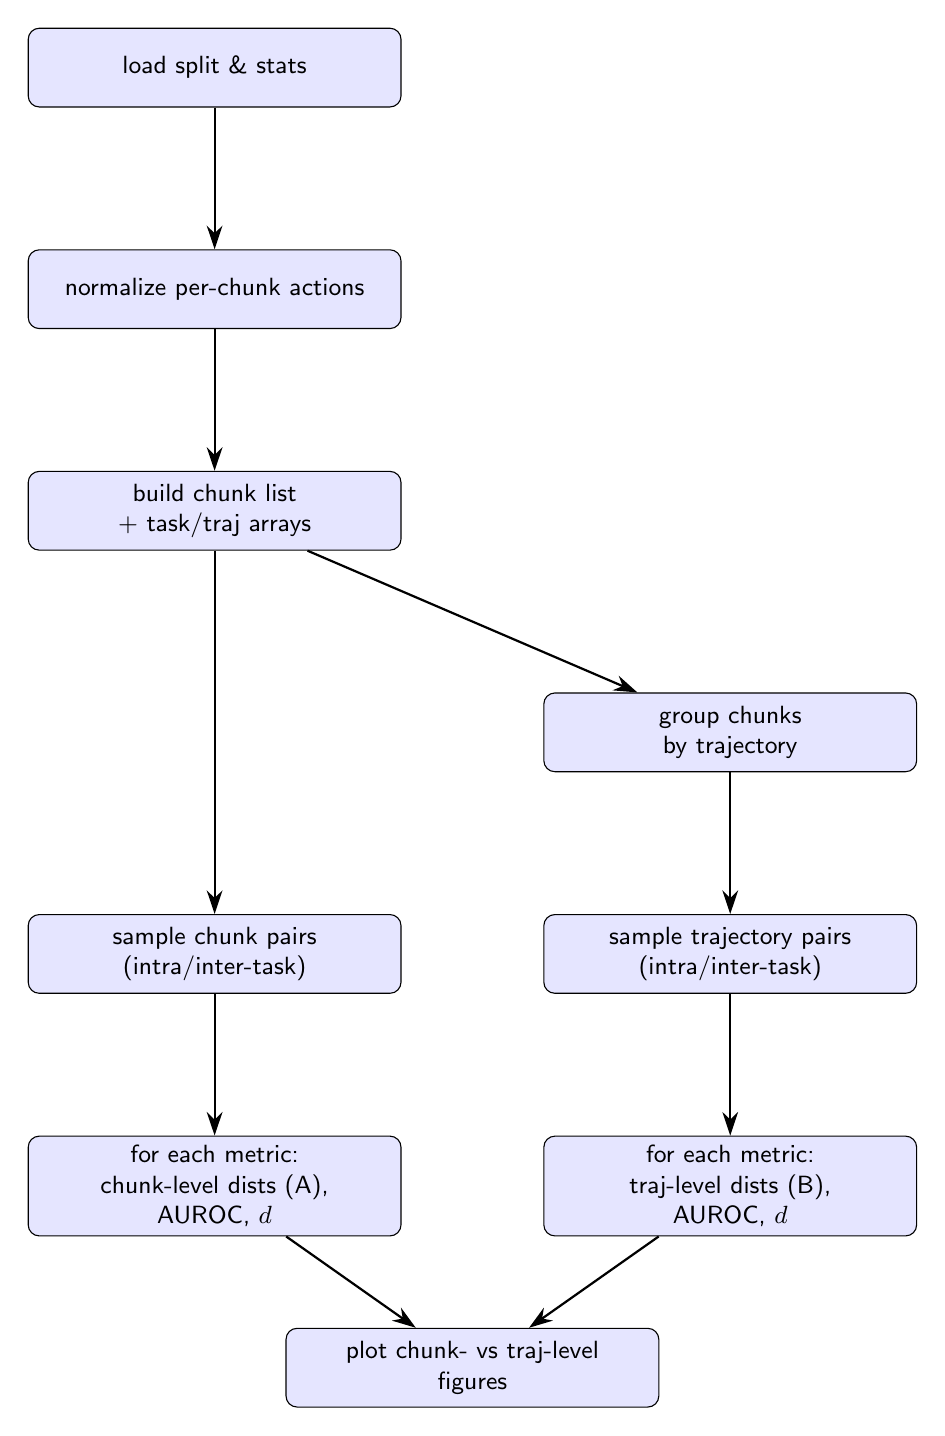
\begin{tikzpicture}[
  node distance=1.8cm and 1.8cm,
  block/.style={
    rectangle,
    draw,
    fill=blue!10,
    text width=4.5cm,
    align=center,
    rounded corners,
    minimum height=1.0cm,
    font=\small\sffamily
  },
  arrow/.style={-{Stealth[length=3mm, width=2mm]}, thick}
]

  % Nodes
  \node (A) [block]                    {load split \& stats};
  \node (B) [block, below=of A]       {normalize per-chunk actions};
  \node (C) [block, below=of B]       {build chunk list \\ + task/traj arrays};

  \node (E) [block, below right=of C]  {group chunks \\ by trajectory};
  \node (D) [block, below left=of E] {sample chunk pairs \\ (intra/inter-task)};

  \node (F) [block, below=of E]       {sample trajectory pairs \\ (intra/inter-task)};
  \node (G) [block, below=of D]       {for each metric: \\ chunk-level dists (A), \\ AUROC, $d$};

  \node (H) [block, below=of F]       {for each metric: \\ traj-level dists (B), \\ AUROC, $d$};

  \coordinate (mid) at ($(G)!0.5!(H)$);
  \node (I) [block, below=of mid]     {plot chunk- vs traj-level \\ figures};

  % Arrows
  \draw [arrow] (A) -- (B);
  \draw [arrow] (B) -- (C);
  \draw [arrow] (C) -- (D);
  \draw [arrow] (C) -- (E);
  \draw [arrow] (D) -- (G);
  \draw [arrow] (E) -- (F);
  \draw [arrow] (F) -- (H);
  \draw [arrow] (G) -- (I);
  \draw [arrow] (H) -- (I);

\end{tikzpicture}
\caption{Metrics task-discriminative validity check for expert trajectories}
\label{fig:trajectory_distinctive_check}
\end{figure}

The proposed metrics are used to compare the matching degree between the generated trajectory and the corresponding task's dataset trajectory. Low-quality trajectories should have poor metrics. For high-quality trajectories, even with differences in waypoints and times, the metric value should be satisfying. This experiment bypasses the model, directly sampling trajectories from different tasks in the dataset to simulate low-quality trajectories, and trajectories from the same task to simulate high-quality trajectories. If a metric cannot tell that two ground-truth trajectories of the same LIBERO-Goal task are more similar to each other than to trajectories of a different task, it carries no task information and cannot measure action quality at all. This is a model-independent property of the metric on the data, and a necessary condition for everything that follows, and is exactly the standard RQ1 (\S\ref{sec:rq1}) asks about.

A metric computed on a single $H$-step chunk is a high-variance, low-context sample of a trajectory that may span hundreds of steps. Two aggregation strategies were compared before adopting one for the checkpoint-level score $\bar m(k)$: \textbf{(A) single-chunk}, which scores one chunk in isolation, the atomic unit an online chunking rollout actually executes; and \textbf{(B) trajectory-level}, which represents a trajectory by its ordered sequence of non-overlapping $H$-step chunks and compares two trajectories window-by-window at aligned positions, averaging the per-window distance.

Neither estimator's quality can be assumed; both should first satisfy a prerequisite that is model-independent and precedes any question about success correlation: a validation distance is uninformative about action quality unless it can already tell that two ground-truth trajectories of the same task are more similar to one another than to trajectories of a different task. This is measured directly. Held-out chunks are partitioned by task and source trajectory; for each metric, this work draws $N_{\mathrm{intra}}$ pairs of chunks from the same task but different trajectories, and $N_{\mathrm{inter}}$ pairs from different tasks, and computes
\begin{equation}
  \mathrm{AUROC} = \Pr\big(d_{\mathrm{inter}} > d_{\mathrm{intra}}\big),
  \qquad
  d_{\mathrm{Cohen}} = \frac{\mu_{\mathrm{inter}}-\mu_{\mathrm{intra}}}{\sigma_{\mathrm{pooled}}},
  \label{eq:taskdisc}
\end{equation}
where $\mathrm{AUROC}=0.5$ indicates chance separation (no task information in the metric) and $\mathrm{AUROC}=1.0$ indicates perfect separation. This test is applied identically under estimators (A) and (B), and the estimator that proves more task-discriminative on ground truth --- (B), as \S\ref{sec:results-taskdisc} shows --- is adopted for every $\bar m(k)$. The workflow is visualized in Figure~\ref{fig:trajectory_distinctive_check}; the resulting distance distributions are shown in Figures~\ref{fig:taskdisc-chunk} and~\ref{fig:taskdisc-traj}.

\paragraph{Implementation setting.} Each of the $428$ ground-truth action trajectories ($10$ LIBERO-Goal tasks, median length $105$ steps) is partitioned into contiguous, non-overlapping $H{=}50$ action chunks by a fixed stride-$H$ tiling ($t_0 = 0, 50, 100, \dots$, so the chunks are a deterministic partition rather than random samples; the sub-$H$ tail is discarded), capped at three chunks per trajectory so that long trajectories do not dominate --- a cap that truncates only $18/428$ trajectories, since the median trajectory yields just two chunks. Every chunk is train-normalized (mean/std estimated on the training split only) and tagged by its task and source trajectory. Per metric draw $3000$ intra-task pairs (same task, but different trajectories --- same-trajectory pairs are excluded so temporally overlapping chunks cannot trivially inflate similarity) and $3000$ inter-task pairs (different tasks), and quantify separation by Eq.~\ref{eq:taskdisc}. The resulting AUROC/Cohen's $d$ values are reported as the RQ1 results in \S\ref{sec:results-taskdisc}.

\subsection{RQ2 Design: Selection Rule and Correlation/Regret Standard}
\label{sec:design-rq2}

RQ2's standard is already made precise in \S\ref{sec:method}: the early-stopping rule of Eq.~\ref{eq:selection} turns a checkpoint-level score $\bar m(k)$ into a single selected checkpoint $k_m^\star$, and Eq.~\ref{eq:rho-regret} scores that selection, together with the whole ranking $\bar m(k)$ induces, against closed-loop success via Spearman's $\rho_m$ and selection regret. No additional design choice is needed beyond fixing, once, which action-chunk generation mode and which aggregation estimator feed $\bar m(k)$ --- both fixed above in \S\ref{sec:implementation-mode} and \S\ref{sec:method-taskdisc} respectively --- so that every metric in every run is scored under an identical protocol.

The implementation-specific settings this experiment relies on are the shared setup of \S\ref{sec:implementation-benchmark}--\S\ref{sec:implementation-sim}: in particular the evaluation mode and metric instantiation (\S\ref{sec:implementation-mode}) that generates $A_k$ for each checkpoint, and the checkpoint-selection and simulator-evaluation pipeline (\S\ref{sec:implementation-pipeline}--\S\ref{sec:implementation-sim}) that computes $k_m^\star$ and obtains $Q(k_m^\star)$ for it. RQ2 is thereby evaluated identically across all five runs of Table~\ref{tab:runs}, so that any asymmetry in the result is attributable to architecture or training-set size rather than to a difference in protocol.

\subsection{RQ3 Design: The Plateau Regime and a Restriction-of-Range Diagnostic}
\label{sec:method-plateau}

A single $\rho_m$ computed over an entire training run conflates two qualitatively different regimes: an early regime in which both $\bar m(k)$ and $Q(k)$ change rapidly as the policy leaves initialization, and a later, converged regime in which $\bar m(k)$ has plateaued and any residual variation in $Q(k)$ is plausibly dominated by simulator evaluation noise. To separate the two, each run's knee is defined as the first checkpoint at which DTW has completed $90\%$ of its total descent,
\begin{equation}
  k_{\mathrm{knee}} = \min\Big\{k : \bar m_{\mathrm{DTW}}(k) \le m_{\min} + 0.1\big(\bar
  m_{\mathrm{DTW}}(0)-m_{\min}\big)\Big\}, \qquad m_{\min}=\min_j \bar m_{\mathrm{DTW}}(j).
  \label{eq:knee}
\end{equation}
$\rho_{\mathrm{DTW}}$ is then recomputed twice: once over the full evaluated range, and once restricted to $\{k\ge k_{\mathrm{knee}}\}$, the converged plateau. A metric that is only a coarse regime-separator (untrained vs. converged) will show a large drop between the two; a metric that retains fine-grained discriminative power inside the plateau will not. This diagnostic is what allows the results in \S\ref{sec:results-plateau} to distinguish ``the metric stopped tracking success'' from ``the evaluation schedule under-sampled a noisy, low-signal region.''

This diagnostic is also how RQ3's second sub-question --- whether genuine overtraining occurs --- is implemented: the deliberately small $150$-trajectory runs of \S\ref{sec:implementation-runs} (SmolVLA-150, OpenVLA-150, and, most aggressively, $\pi_{0.5}$-150) exist specifically to stress-test for a post-knee decline in $Q(k)$ that a metric would need to catch, and $\pi_{0.5}$-150's simulator-evaluation schedule was deliberately extended past its apparent peak (Table~\ref{tab:runs}, Sim.\ evals) to check whether an early apparent decline was a genuine downturn or a restriction-of-range artifact.

\subsection{RQ4 Design: Bootstrap Confidence Intervals}
\label{sec:method-bootstrap}

Every $\rho_m$ above is a point estimate computed from as few as $11$ and at most $33$ simulator evaluations per run, each itself a $\pm5\%$-noisy $100$-episode Bernoulli success-rate estimate. Ranking metrics directly by these point estimates risks over-interpreting sampling noise. This work attaches a percentile bootstrap confidence interval to every $\rho_m$ \cite{efron1979bootstrap,efron1993bootstrap}: for each run, its evaluated checkpoints are resampled with replacement $B=10{,}000$ times, a tie-corrected Spearman correlation is recomputed on each resample, and the central $95\%$ interval is reported together with $\Pr(\rho_m>0)$. To compare two metrics within a
run without their mutual correlation confounding the test, the \emph{same} bootstrap resample is used for both and the paired difference $\Delta\rho=\rho_A-\rho_B$ is reported over the checkpoints they share.
This yields three tiers of claim, from weakest to strongest: a metric's point-estimate $\rho_m$; whether that $\rho_m$'s CI excludes zero (a significant association with success); and whether a paired $\Delta\rho$ CI excludes zero (a significant \emph{ordering} between two metrics). Only the last licenses a claim of the form ``metric $A$ is better than metric $B$'' --- the standard RQ4 (\S\ref{sec:rq4}) applies to every comparison in \S\ref{sec:results-bootstrap}. No additional implementation setting is required beyond the sparse simulator-evaluation counts $n$ already fixed per run in \S\ref{sec:implementation-sim} (Table~\ref{tab:runs}), since it is precisely that sparsity the bootstrap procedure is designed to quantify.

\subsection{RQ5 Design: Selecting the Replan Horizon Across Checkpoints}
\label{sec:design-rq5}

RQ5 is evaluated on SmolVLA-150, at five checkpoints spanning the run's full quality range (peak $Q\in\{0.30,0.48,0.58,0.63,0.68\}$), so that a metric's ability to select $h$ can be distinguished from $h$ merely being favorable at one $\theta_k$. At each checkpoint, $Q(h)$ is measured on a shared grid $h\in\{1,3,5,10,15,25,50\}$ (a superset added at the two extreme-quality checkpoints), under the identical protocol used for every $Q(k)$ elsewhere in this thesis --- same tasks, seed, and episode count at every $h$, so that episodes are paired across the grid.

Every offline predictor here is a function of the same cached quantity: writing $P[t,k]$ for the $k$-th action of the chunk $\pi_k$ predicts from the observation at time $t$ (so $P[t,0]$ is $\pi_k$'s immediate action and $A_k$ of \S\ref{sec:method-notation} is the row $P[t,\cdot]$), the predicted chunk is cached at every held-out validation frame with $H{=}50$; two independent samples are drawn per frame to isolate the flow-matching sampler's own noise from genuine plan revision. Under a replanning schedule with horizon $h$, the policy re-samples a fresh chunk every $h$ steps and executes only its first $h$ actions before doing so,
\begin{equation}
  a_{\mathrm{exec}}(t_0{+}j) = P\big[\,t_0+h\lfloor j/h\rfloor,\;\; j\bmod h\,\big].
  \label{eq:aexec}
\end{equation}
Three families of predictor are compared, all as functions of $h$ alone at a fixed checkpoint.

\paragraph{Truncated prefix.} The chunk-position error at offset $k$ is $e_k=\mathbb E_t\lVert P[t,k]-a^\star_{t+k}\rVert_2^2$; truncating the predicted chunk to its first $h$ steps and averaging gives
\begin{equation}
  \bar m_{\mathrm{prefix}}(h) = \frac1h\sum_{k=0}^{h-1} e_k,
  \label{eq:prefix}
\end{equation}
an extension of Eq.~\ref{eq:dtw}--\ref{eq:cos} requiring no new machinery, but one that compares sequences of length $h$ against each other across the grid, so $\bar m_{\mathrm{prefix}}(h)$ is not on a common scale from one $h$ to the next.

\paragraph{Fixed-window stitch.} Holding the comparison window at $H$ instead, and building the executed sequence $\hat A_h(t)=\big(a_{\mathrm{exec}}(t),\dots,a_{\mathrm{exec}}(t{+}H{-}1)\big)$ from Eq.~\ref{eq:aexec} under a replanning schedule of horizon $h$, gives
\begin{equation}
  \bar m_{\mathrm{stitch}}(h) = \mathbb E_t\, D\big(\hat A_h(t),\, A^\star_t\big),
  \qquad D\in\{D_{\mathrm{DTW}},\,D^\varepsilon_{\mathrm{OT}},\,D_{\cos},\,L_1,\,L_2\},
  \label{eq:stitch}
\end{equation}
using the same distances $D$ as \S\ref{sec:method-metrics}. Because every $\hat A_h(t)$ and $A^\star_t$ has the same length $H$ regardless of $h$, only the replanning schedule varies across the grid, removing the scale confound of Eq.~\ref{eq:prefix}.

\paragraph{Switching cost.} A replan at $j{=}h$ discards the stale continuation of the previous chunk in favor of a freshly sampled one; the resulting discontinuity, relative to the step size the ground-truth trajectory itself takes, is
\begin{equation}
  \bar m_{\mathrm{switch}}(h) = \mathbb E_t\Big[\big\lVert P[t{+}h,0]-P[t,h{-}1]\big\rVert_2^2\Big]
  - \mathbb E_t\Big[\big\lVert a^\star_{t+h}-a^\star_{t+h-1}\big\rVert_2^2\Big],
  \label{eq:switch}
\end{equation}
which isolates the discontinuity effect from the accuracy term of Eq.~\ref{eq:prefix}--\ref{eq:stitch} and, taken alone, is minimized by never replanning ($h{\to}H$). A $\lambda$-free composite instead sums the two effects at matched, per-step scale, $\bar m_{\mathrm{stitch},L_2}(h) + \bar m_{\mathrm{switch}}(h)/h$, with no tuned weight between them since both terms are already mean-squared, normalized-action quantities.

Because $h$ ranges over a small, non-monotone discrete grid rather than a training curve, the selection rule of Eq.~\ref{eq:selection} does not apply as stated; $h_m^\star$ is instead the direct minimizer, $h_m^\star=\arg\min_h \bar m(h)$, and Eq.~\ref{eq:rho-regret}'s $\rho_m$ and regret are computed with $h$ in place of $k$. A metric with no $h$-dependence (any checkpoint-level offline metric of \S\ref{sec:method-metrics}, evaluated once rather than per horizon) is charged the regret of a uniform random choice over the grid, giving an explicit null against which every candidate is compared.

\clearpage

\section{Results}
\label{sec:results}

This section reports, in the order the questions were posed in \S\ref{sec:rq} and designed in \S\ref{sec:implementation}, the outcome of each of the five experiments, and closes in \S\ref{sec:results-conclusions} by answering each research question directly.

\subsection{RQ1 Results: Task-Discriminative Validity}
\label{sec:results-taskdisc}

Applying the design and sampling procedure of \S\ref{sec:method-taskdisc} to the LIBERO-Goal held-out trajectories gives the following separation strengths, quantified by AUROC and Cohen's $d$ (Eq.~\ref{eq:taskdisc}), where $\mathrm{AUROC}=0.5$ is chance (no task information) and $1.0$ is perfect task separation.

\begin{figure}[!htb]
  \centering
  \includegraphics[width=\textwidth]{figures/task_discriminative_validity_chunk.png}
  \caption{\textbf{Single-chunk (atomic) distances.} Intra-task (blue) vs.\ inter-task (orange)
  distance distributions per metric, drawn as outlined step histograms. The bottom-right
  panel (shared with Fig.~\ref{fig:taskdisc-traj}) contrasts single-chunk (green) with trajectory-level (purple) AUROC.}
  \label{fig:taskdisc-chunk}
\end{figure}

\begin{figure}[!htb]
  \centering
  \includegraphics[width=\textwidth]{figures/task_discriminative_validity_traj.png}
  \caption{\textbf{Trajectory-level (phase-aligned, window-averaged) distances}, same axes and metrics as Fig.~\ref{fig:taskdisc-chunk}. Representing each trajectory by its ordered chunks and comparing two entire trajectories window-by-window}
  \label{fig:taskdisc-traj}
\end{figure}

\paragraph{Single-chunk vs. Trajectory level}
Every metric clears chance under both estimators, but the two differ sharply in strength. The single chunk (A) separates tasks only moderately (AUROC $0.65$--$0.69$), because LIBERO-Goal's ten tasks share a large common motion vocabulary --- reach, grasp, transport --- so an arbitrary $50$-step window overlaps heavily across tasks. The trajectory-level, phase-aligned estimator (B) is decisively stronger: every metric rises to AUROC $\ge0.90$ and Cohen's $d$ roughly triples. The improvement is attributable specifically to phase alignment rather than variance reduction alone --- e.g.\ DTW's intra-task mean distance falls from $7.06$ to $1.84$ under (B) while its inter-task mean barely moves ($10.23\to8.27$), consistent with comparing corresponding motion phases rather than arbitrary ones. On this basis, estimator (B) is adopted for every $\bar m(k)$ in the remainder of this chapter, and the RQ1 precondition of \S\ref{sec:method-taskdisc} is satisfied for all five candidate metrics.


\begin{table}[H]
\centering
\caption{\textbf{Estimator (A), single-chunk.} Intra- vs.\ inter-task distances between ground-truth $H{=}50$ action chunks ($3000$ cross-trajectory pairs each), sorted by AUROC.}
\label{tab:taskdisc-chunk}
\begin{tabular}{lrrrr}
\toprule
Metric & mean intra & mean inter & AUROC & Cohen's $d$ \\
\midrule
OT  & 6.625 & 10.182 & 0.692 & 0.62 \\
DTW & 7.063 & 10.230 & 0.677 & 0.47 \\
L1  & 0.772 & 0.965  & 0.660 & 0.56 \\
COS & 0.688 & 0.922  & 0.657 & 0.66 \\
L2  & 1.420 & 1.843  & 0.653 & 0.39 \\
\bottomrule
\end{tabular}
\end{table}

\begin{table}[H]
\centering
\caption{\textbf{Estimator (A) single-chunk vs.\ (B) trajectory-level} (phase-aligned, window-averaged) task separation, $3000$ cross-trajectory pairs each. }
\label{tab:taskdisc-traj}
\begin{tabular}{lrrrr}
\toprule
 & \multicolumn{2}{c}{chunk (single $H{=}50$)} & \multicolumn{2}{c}{trajectory (window-avg)} \\
\cmidrule(lr){2-3}\cmidrule(lr){4-5}
Metric & AUROC & Cohen's $d$ & AUROC & Cohen's $d$ \\
\midrule
COS & 0.657 & 0.66 & 0.927 & 2.19 \\
OT  & 0.692 & 0.62 & 0.923 & 1.68 \\
DTW & 0.677 & 0.47 & 0.911 & 1.61 \\
L2  & 0.653 & 0.39 & 0.903 & 1.70 \\
L1  & 0.660 & 0.56 & 0.901 & 1.80 \\
\bottomrule

\end{tabular}
\end{table}

RQ1's answer is therefore affirmative for every candidate metric under estimator (B): none is disqualified, so \S\ref{sec:results-crossmodel}--\S\ref{sec:results-bootstrap} may proceed to test whether that same estimator predicts closed-loop success.

\subsection{RQ2 Results: Closed-Loop Success Across Checkpoints}
\label{sec:results-runs}

\begin{table}[H]
\centering
\caption{The five fine-tuning runs. All LIBERO-Goal, LoRA $r{=}32$; $Q(k)$ is $100$-episode simulated
success.}
\label{tab:runs}
\begin{tabular}{lllrrr}
\toprule
Run & Architecture & Train traj. & Checkpoints & Sim.\ evals & Peak $Q$ \\
\midrule
SmolVLA-150      & flow-matching (450M) & 150 & 200 (to 100k) & 35 & 0.68 \\
OpenVLA-150      & discrete-token (7B)  & 150 & 79 (to 39.5k) & 19 & 0.83 \\
OpenVLA-full     & discrete-token (7B)  & 342 & 68 (to 34k)   & 11 & 0.78 \\
$\pi_{0.5}$-full & flow-matching (4B)   & 342 & 147 (to 73.5k)$^\ddagger$& 32 & 0.18$^\dagger$ \\
$\pi_{0.5}$-150  & flow-matching (4B)   & 150 & 80 (to 40k)   & 28 & 0.38$^\dagger$ \\
\bottomrule
\end{tabular}
\\[2pt]
{\footnotesize $^\ddagger$ $\pi_{0.5}$-full logged offline metrics to step $73499$, but its last
simulator rollout is at $52499$; checkpoint selection for this run is therefore restricted to
$k\le52499$, so that no reported $k_m^\star$ lies outside the range in which $Q$ was measured
(Table~\ref{tab:rankings}). \\
$^\dagger$ The two $\pi_{0.5}$ runs are evaluated at different replanning horizons: $\pi_{0.5}$-150 at $n_{\mathrm{action}}{=}10$ and $\pi_{0.5}$-full at $n_{\mathrm{action}}{=}50$ (the full predicted chunk executed blind before replanning), and the longer horizon roughly halves LIBERO success relative to shorter ones; only the relative ranking of metrics is meaningful for these two rows, not the absolute success level.}
\end{table}

Full validation metrics and corresponding checkpoint success rate data are visualized in Appendix~\ref{app:figures}.

\subsection{RQ2 Results: Cross-Model Correlation with Closed-Loop Success}
\label{sec:results-crossmodel}

\begin{figure}[h]
  \centering
  \includegraphics[width=0.92\textwidth]{figures/crossmodel_early_stopping.png}
  \caption{Spearman $\rho_m$ of every offline metric with LIBERO-Goal success, by run (left), and the corresponding success curve $Q(k)$ over training (right). Trajectory (DTW/OT/cosine) and regression ($L_1$/$L_2$) metrics are positive in every run; the likelihood/loss family (NLL, or the flow-matching loss standing in for it) splits by architecture, positive and significant for the two discrete-token runs, weak or statistically indistinguishable from zero for the flow-matching runs
  (\S\ref{sec:results-bootstrap}).}
  \label{fig:crossmodel}
\end{figure}

Figure~\ref{fig:crossmodel} summarizes the headline result across all five runs and all applicable metrics. Ordering the five runs SmolVLA-150 / OpenVLA-150 / OpenVLA-full / $\pi_{0.5}$-full /
$\pi_{0.5}$-150, the trajectory-similarity metrics are positive throughout: $\rho_{\mathrm{DTW}} =
0.72/0.75/0.85/0.90/0.72$, $\rho_{\mathrm{OT}} = 0.62/0.84/0.66/0.89/0.68$, and $\rho_{\cos} =
0.68/0.75/0.89/0.86/0.77$. DTW in particular is never negative across the five runs and its selection
regret never exceeds $0.17$, a first empirical basis for the conclusion drawn in
\S\ref{sec:results-conclusions}\ref{conc:correlation}.

\subsection{RQ2 Results: Per-Model Metric Rankings}
\label{sec:results-permodel}

Table~\ref{tab:rankings} reports, per run, every applicable metric's selected checkpoint $k_m^\star$, Spearman correlation $\rho_m$, and selection regret, sorted by $\rho_m$.

\begin{table}[h]
\centering
\caption{Per-run metric rankings: selected checkpoint, Spearman $\rho_m$, and selection regret
(Eq.~\ref{eq:selection}--\ref{eq:rho-regret}). Because $Q$ is measured only at the sparse
sim-evaluated checkpoints of Table~\ref{tab:runs}, $Q(k_m^\star)$ is read at the evaluated
checkpoint nearest $k_m^\star$; the selection range of each run is restricted to its
sim-evaluated range so that this substitution is never more than one evaluation interval
($\le1500$ steps in every row above). For $\pi_{0.5}$-full, whose offline metrics run to step
$73499$ but whose last rollout is at $52499$, this restriction is what makes its regret column
interpretable at all (\S\ref{sec:results-permodel}).}
\label{tab:rankings}
\begin{minipage}[t]{0.48\textwidth}
\centering \textbf{OpenVLA-full} (342 traj.)\\[2pt]
\begin{tabular}{lrrr}
\toprule
Metric & $k_m^\star$ & $\rho$ & Regret \\ \midrule
Cosine & 28499 & $+0.89$ & 0.05 \\
DTW    & 21499 & $+0.85$ & 0.00 \\
$L_2$  & 21499 & $+0.85$ & 0.00 \\
$L_1$  & 29999 & $+0.85$ & 0.05 \\
CE     & 33999 & $+0.83$ & 0.04 \\
Acc.   & 33999 & $+0.83$ & 0.04 \\
NLL    & 33999 & $+0.83$ & 0.04 \\
OT     & 33999 & $+0.66$ & 0.04 \\
\bottomrule
\end{tabular}
\end{minipage}
\hfill
\begin{minipage}[t]{0.48\textwidth}
\centering \textbf{OpenVLA-150} (discrete-token)\\[2pt]
\begin{tabular}{lrrr}
\toprule
Metric & $k_m^\star$ & $\rho$ & Regret \\ \midrule
OT     & 33499 & $+0.84$ & 0.08 \\
Acc.   & 37499 & $+0.78$ & 0.02 \\
$L_1$  & 30999 & $+0.78$ & 0.06 \\
DTW    & 23499 & $+0.75$ & 0.17 \\
Cosine & 23499 & $+0.75$ & 0.17 \\
$L_2$  & 23499 & $+0.75$ & 0.17 \\
CE     & 30999 & $+0.72$ & 0.06 \\
NLL    & 30999 & $+0.72$ & 0.06 \\
\bottomrule
\end{tabular}
\end{minipage}

\vspace{1em}

\begin{minipage}[t]{0.48\textwidth}
\centering \textbf{$\pi_{0.5}$-full} (flow-matching, 342 traj.)\\[2pt]
\begin{tabular}{lrrr}
\toprule
Metric & $k_m^\star$ & $\rho$ & Regret \\ \midrule
DTW    & 39499 & $+0.90$ & 0.01 \\
OT     & 39499 & $+0.89$ & 0.01 \\
Cosine & 39499 & $+0.86$ & 0.01 \\
$L_1$  & 43499 & $+0.84$ & 0.03 \\
$L_2$  & 46499 & $+0.81$ & 0.06 \\
NLL/FM & 31999 & $+0.46$ & 0.08 \\
\bottomrule
\end{tabular}
\end{minipage}
\hfill
\begin{minipage}[t]{0.48\textwidth}
\centering \textbf{$\pi_{0.5}$-150} (overtraining stress run)\\[2pt]
\begin{tabular}{lrrr}
\toprule
Metric & $k_m^\star$ & $\rho$ & Regret \\ \midrule
$L_1$  & 31999 & $+0.78$ & 0.05 \\
Cosine & 39499 & $+0.77$ & 0.04 \\
$L_2$  & 37999 & $+0.73$ & 0.08 \\
DTW    & 33499 & $+0.72$ & 0.07 \\
OT     & 24499 & $+0.68$ & 0.17 \\
NLL/FM &  8999 & $-0.16$ & 0.20 \\
\bottomrule
\end{tabular}
\end{minipage}

\vspace{1em}
\centering
\begin{minipage}[t]{0.48\textwidth}
\centering \textbf{SmolVLA-150} (flow-matching)\\[2pt]
\begin{tabular}{lrrr}
\toprule
Metric & $k_m^\star$ & $\rho$ & Regret \\ \midrule
$L_1$  & 56000 & $+0.77$ & 0.15 \\
DTW    & 22000 & $+0.72$ & 0.17 \\
$L_2$  & 24500 & $+0.70$ & 0.14 \\
Cosine & 33000 & $+0.68$ & 0.16 \\
OT     & 11000 & $+0.62$ & 0.20 \\
NLL/FM & 13000 & $-0.35$ & 0.14 \\
\bottomrule
\end{tabular}
\end{minipage}
\end{table}




Two mechanistic points follow from Table~\ref{tab:rankings}. First, the metrics available depend on architecture: only OpenVLA exposes cross-entropy loss and token accuracy, since only a discrete-token policy has them; the flow-matching policies retain $L_1$/$L_2$ regression error, which is on par with or above their own DTW score in every flow-matching run. Second, on OpenVLA-full, $L_2$ and DTW select the identical checkpoint ($k^\star=21499$) with identical $\rho$ and zero regret, foreshadowing the statistical indistinguishability of the trajectory and regression families confirmed in \S\ref{sec:results-bootstrap}.

Two properties of the regret column deserve stating, since both limit what may be read off it. The
first is that regret is only defined up to the resolution of the simulator-evaluation grid. A metric
may select any of a run's $68$--$200$ logged checkpoints, but $Q$ exists at only $11$--$35$ of them,
so $Q(k_m^\star)$ is in general read at the nearest evaluated checkpoint rather than at
$k_m^\star$ itself. Inside the evaluated range this substitution is bounded by one evaluation
interval and is harmless; a selection that falls \emph{outside} it, however, is not scored but
extrapolated, and several distinct selections can then collapse onto one shared measurement and one
shared regret value. $\pi_{0.5}$-full is the one run where this can arise, since its metrics extend
$21{,}000$ steps past its last rollout: selecting over the untruncated curve places DTW, OT, cosine,
$L_1$ and $L_2$ at steps $55999$--$60499$, all of which are scored by the single rollout at $52499$
and so receive an identical, uninformative regret of $0.04$. Restricting its selection range to the
evaluated range (Table~\ref{tab:runs}$^\ddagger$) removes the extrapolation and separates the five
metrics ($0.01$/$0.01$/$0.01$/$0.03$/$0.06$), and no row of Table~\ref{tab:rankings} is then scored
more than $1500$ steps from its selected checkpoint.
The second is that regret inherits the dynamic range of its run's success curve. On $\pi_{0.5}$-full,
peak $Q$ is only $0.18$ and the converged band spans roughly $0.12$--$0.18$, so the entire
achievable regret spread is comparable to the $\pm5\%$ sampling noise of a $100$-episode evaluation
(\S\ref{sec:implementation-benchmark}); differences of a few points in that run's regret column are
not evidence of a metric ordering. $\pi_{0.5}$-150 (peak $0.38$, regret spread $0.04$--$0.20$) and
the two OpenVLA runs are where the regret statistic has the range to discriminate.

Taken together with Figure~\ref{fig:crossmodel}, RQ2's answer is affirmative and architecture-general: DTW, OT, and cosine distance are positive predictors of closed-loop success in every one of the five runs, so an offline trajectory-similarity metric can substitute for a rollout when selecting among checkpoints, subject to the statistical qualifications of RQ4 (\S\ref{sec:results-bootstrap}).

\subsection{RQ3 Results: Plateau Regime, Restriction of Range, and the Overtraining Check}
\label{sec:results-plateau}

\begin{table}[h]
\centering
\caption{DTW$\to$success Spearman $\rho$ over the full evaluated range vs.\ restricted to the converged
plateau $\{k\ge k_{\mathrm{knee}}\}$ (Eq.~\ref{eq:knee}). Both $\rho$ columns are computed only over
checkpoints carrying both a DTW value and a $Q(k)$, so ``plateau pts'' counts sim-evaluated
checkpoints past the knee, not logged ones; for $\pi_{0.5}$-full the DTW curve is truncated at
step $52499$ as in Table~\ref{tab:rankings}, which is what places its knee at $14499$.}
\label{tab:plateau}
\begin{tabular}{lrrrrr}
\toprule
Run & $k_{\mathrm{knee}}$ & Plateau pts & $\rho_{\mathrm{full}}$ & $\rho_{\mathrm{plateau}}$ & Drop \\
\midrule
SmolVLA-150      &  4500 & 30/35 & $+0.72$ & $+0.55$ & 0.17 \\
OpenVLA-150      &  6999 & 16/19 & $+0.75$ & $+0.59$ & 0.16 \\
OpenVLA-full     &  8499 &  9/11 & $+0.86$ & $+0.73$ & 0.12 \\
$\pi_{0.5}$-full & 14499 & 25/32 & $+0.91$ & $+0.81$ & 0.10 \\
$\pi_{0.5}$-150  &  9999 & 22/28 & $+0.72$ & $\mathbf{+0.43}$ & $\mathbf{0.29}$ \\
\bottomrule
\end{tabular}
\end{table}

\begin{figure}[h]
  \centering
  \includegraphics[width=0.92\textwidth]{figures/plateau_restriction.png}
  \caption{\textbf{Left:} DTW$\to$success $\rho$, full range vs.\ converged plateau, all five runs.
  \textbf{Right:} $\pi_{0.5}$-150's validation DTW (converges early, axis inverted) against its success
  curve (a noisy, low-ceiling band that dips near $20$k training steps and recovers to a $38\%$ peak by
  $34$k once training is extended to $40$k steps).}
  \label{fig:plateau}
\end{figure}

$\rho_{\mathrm{full}}\ge\rho_{\mathrm{plateau}}$ holds for every run (Table~\ref{tab:plateau}): the offline metrics are, at minimum, reliable regime separators (untrained vs.\ converged), and fine-ranking already-converged checkpoints is strictly harder. The knee itself should be read as a property of the observed curve rather than of the run: Eq.~\ref{eq:knee} locates it at $90\%$ of DTW's \emph{measured} total descent, so truncating a curve raises its observed minimum and moves the knee earlier. $\pi_{0.5}$-full is the case in point --- restricting it to its sim-evaluated range (\S\ref{sec:results-permodel}) moves $k_{\mathrm{knee}}$ from $18999$ to $14499$ and adds three checkpoints to its plateau, while leaving $\rho_{\mathrm{plateau}}$ essentially unchanged ($+0.80\to+0.81$). The diagnostic is therefore robust to where the curve is cut even though the knee step is not. For four of the five runs the plateau correlation remains usable ($\rho_{\mathrm{plateau}}\ge0.55$), so the metric retains real discriminative power even inside the plateau. $\pi_{0.5}$-150 is the exception, dropping to
$\rho_{\mathrm{plateau}}=+0.43$. Critically, this is a restriction-of-range artifact rather than genuine action-quality overtraining: an earlier $20{,}000$-step view of this run showed success falling from $31\%$ to $23\%$ after its peak, consistent with overtraining, but extending training to $40{,}000$ steps shows success recovering to a $38\%$ peak (Figure~\ref{fig:plateau}, right) --- so the apparent decline was an artifact of stopping mid-dip in a low-ceiling, noisy success band whose spread is comparable to the $\pm5\%$ sampling noise of a $100$-episode evaluation, not a monotone downturn. The practical implication, developed into a conclusion in \S\ref{sec:results-conclusions}\ref{conc:plateau}, is that these metrics support a coarse but robust early-stopping decision (do not stop before the knee) even where they cannot reliably fine-rank checkpoints once training has converged.

RQ3's two sub-questions are therefore answered together: metric-based early stopping is effective at the coarse grain that matters most (never stopping before the knee, at low regret), but none of the three $150$-trajectory runs designed to induce it ultimately exhibits a genuine, sustained action-quality decline, so this experiment cannot show how these metrics would behave under real overtraining.

\subsection{RQ4 Results: Statistical Power and Bootstrap Confidence Intervals}
\label{sec:results-bootstrap}

\begin{table}[h]
\centering
\caption{Bootstrap $95\%$ confidence intervals on $\rho$ ($B{=}10{,}000$ resamples, tie-corrected Spearman, paired checkpoint resampling per Eq.~\ref{eq:rho-regret} and \S\ref{sec:method-bootstrap}). ``\#sig''
counts metrics whose interval excludes $0$; ``best $L$'' is the stronger of $L_1$/$L_2$.}
\label{tab:bootstrap}
\begin{tabular}{lccccc}
\toprule
Run & $n$ & \#sig & DTW $\rho$ [95\% CI] & best $L$ $\rho$ [95\% CI] & NLL $\rho$ [95\% CI] \\
\midrule
SmolVLA-150      & 35 & 5/6 & $0.71\,[0.43,\,0.89]$ & $0.76\,[0.50,\,0.91]$ & $-0.34\,[-0.67,\,0.04]$ \\
OpenVLA-150      & 19 & 8/8 & $0.75\,[0.34,\,0.94]$  & $0.78\,[0.42,\,0.95]$  & $0.72\,[0.33,\,0.92]$ \\
OpenVLA-full     & 11 & 8/8 & $0.84\,[0.46,\,0.99]$  & $0.84\,[0.42,\,0.98]$  & $0.81\,[0.40,\,0.97]$ \\
$\pi_{0.5}$-full & 33 & 6/6 & $0.90\,[0.79,\,0.95]$  & $0.83\,[0.64,\,0.93]$  & $0.41\,[0.01,\,0.70]$ \\
$\pi_{0.5}$-150  & 28 & 5/6 & $0.71\,[0.37,\,0.90]$  & $0.78\,[0.50,\,0.93]$  & $-0.17\,[-0.57,\,0.25]$ \\
\bottomrule
\end{tabular}
\end{table}

Statistical power, not the metric family, is the binding constraint on how strong a claim the data support.
$\pi_{0.5}$-full ($n{=}33$) is powered enough to resolve within-run structure, as its $95\%$ confidence intervals are narrow; DTW's interval spans less than $0.20$.

SmolVLA-150 shows how strongly this depends on evaluation density. Under the original schedule ($n{=}18$), which sampled almost only the post-knee plateau, no metric cleared zero at $95\%$ --- including DTW ($0.47$, CI $[-0.09,0.87]$): this lightweight $450$M model converges so quickly on the small $150$-trajectory dataset that the success rate completes most of its rise within the first few thousand steps, where $Q(k)$ had been measured only about five times, whereas checkpoints and offline metrics were saved every $500$ steps --- so the shortfall was one of evaluation coverage, not training resolution. Densifying the pre-plateau ground truth to $n{=}35$ rollouts removes this restriction of range: every trajectory and regression metric now clears zero (DTW $0.71$, CI $[0.43,0.89]$; best $L$ $0.76$, CI $[0.50,0.91]$), and in the paired test DTW significantly exceeds the flow-matching surrogate NLL/FM ($\Pr{=}1.00$, $\Delta\rho$ CI $[0.64,1.41]$). The earlier non-significance was therefore an artifact of sparse evaluation rather than a genuine failure of the metrics; on the converged plateau itself, however, they still predict success only coarsely (Appendix~\ref{app:figures}).

Within every run, DTW's interval overlaps OT's, cosine's, $L_1$'s, and $L_2$'s: the paired-resampling test finds DTW rank-\emph{identical} to $L_2$ on OpenVLA-full ($\Delta\rho\equiv0$) and finds $\Pr(\rho_{\mathrm{DTW}}>\rho_{L_2})$ indistinguishable from a coin flip on the three intermediate runs ($0.65/0.44/0.33$). DTW significantly outperforms a loss-based metric in exactly one comparison: against the flow-matching surrogate NLL/FM on $\pi_{0.5}$-full ($\Pr=1.00$, $\Delta\rho$ CI $[0.26,0.92]$). The architecture split in NLL's validity is statistically confirmed for OpenVLA (significantly positive in both OpenVLA runs) and, more weakly, for $\pi_{0.5}$-full; for SmolVLA-150 and $\pi_{0.5}$-150 the NLL/FM interval spans zero, so the negative point estimates in those two rows should be read as uninformative, not as evidence of a reliably anti-correlated surrogate.

RQ4's answer is therefore mixed by design: the architecture split between token-NLL and flow-matching-loss is statistically defensible, but most orderings \emph{within} the trajectory/regression family (DTW vs.\ OT vs.\ cosine vs.\ $L_1$/$L_2$) are not resolved at the sample sizes available here.

\subsection{RQ5 Results: The Replan Horizon Is Selectable Offline, Under a Specific Construction}
\label{sec:results-rq5}

\begin{table}[h]
\centering
\caption{RQ5: mean selection regret (success-rate points, lower is better) of representative offline predictors across the five SmolVLA-150 checkpoints, against a metric-blind random-choice null. $h^\star$: the horizon selected at every one of the five checkpoints, where constant.}
\label{tab:replan}
\begin{tabular}{lcc}
\toprule
Predictor family & Mean regret & $h^\star$ (all 5 ckpts) \\
\midrule
$\bar m_{\mathrm{stitch}}$, cosine/$L_2$ & $2.4$ & $15$ \\
$\bar m_{\mathrm{stitch}}$, DTW & $6.6$ & --- \\
$\bar m_{\mathrm{prefix}}$, $L_2$ & $10.8$ & --- \\
\emph{(null) random choice over the grid} & $10.6$ & --- \\
Switching cost only (total variation, jerk) & $19.0$ & $50$ \\
\bottomrule
\end{tabular}
\end{table}

Pooled over the five checkpoints ($n{=}500$ paired episodes per horizon, binomial s.e.\ $2.2$), $Q(h)$ is unimodal with a plateau at $h\in\{10,15\}$ ($51\%$) and every other grid point significantly worse (paired exact binomial, $p\le0.005$), falling to $34\%$ at the fully open-loop $h{=}50$ (Figure~\ref{fig:replan-qh}). The fixed-window construction $\bar m_{\mathrm{stitch}}$ recovers this optimum reliably: its cosine and $L_2$ instantiations select $h{=}15$ at every one of the five checkpoints, for a mean regret of $2.4$ points against the null's $10.6$ (Table~\ref{tab:replan}, Figure~\ref{fig:replan-regret}). The truncated construction $\bar m_{\mathrm{prefix}}$, computed from the identical cached chunks with the identical distance, performs no better than the null ($10.8$): truncating the chunk to $h$ steps compares sequences of different length across the grid, so the score is not on a comparable scale from one $h$ to the next, whereas holding the window fixed at $H$ removes exactly that confound. DTW, the most reliable single default for RQ2's checkpoint selection, is here only middling ($6.6$); it is invariant to temporal warping, which is a liability rather than an asset when the question is precisely \emph{when} an action is issued. Scoring the switching discontinuity alone is actively counterproductive, always selecting the fully open-loop $h{=}50$ --- the single significantly worst point on the grid --- for a mean regret of $19.0$, worse than choosing at random (Figure~\ref{fig:replan-regret}); it is informative only inside the $\lambda$-free composite with a stitched accuracy term, not on its own.

\begin{figure}[h]
  \centering
  \includegraphics[width=0.92\textwidth]{figures/slide_replan_qh.png}
  \caption{RQ5 ground truth. \textbf{Left:} $Q(h)$ per checkpoint; peak success varies with checkpoint quality ($30$--$68\%$) but the shape is consistently unimodal. \textbf{Right:} pooled over the five checkpoints ($n{=}500$/horizon); the shaded band is the $95\%$ CI and $*$ marks horizons significantly worse than the plateau $h\in\{10,15\}$ (paired exact binomial, $p<0.05$).}
  \label{fig:replan-qh}
\end{figure}

\begin{figure}[h]
  \centering
  \includegraphics[width=0.85\textwidth]{figures/slide_replan_regret.png}
  \caption{RQ5: mean selection regret by predictor family across the five checkpoints (Table~\ref{tab:replan}), against the metric-blind random-choice null (dashed). Fixed-window stitched predictors (blue) cluster below the null; truncated-prefix (orange) sits at or above it; smoothness-only (purple) is nearly double it.}
  \label{fig:replan-regret}
\end{figure}

Figure~\ref{fig:replan-alignment} makes the mechanism behind Table~\ref{tab:replan} visible directly: stacked on a shared $h$-axis (never a twin $y$-axis, since the two curves live on unrelated scales), the fixed-window $\bar m_{\mathrm{stitch,cos}}$ curve bottoms out inside the online plateau, $\bar m_{\mathrm{prefix},L_2}$ bottoms out too early, and $\mathrm{tv\_ratio}$ (smoothness only) decreases monotonically toward $h{=}H$ --- the single horizon the online curve rejects most strongly.

\begin{figure}[h]
  \centering
  \includegraphics[width=0.8\textwidth]{figures/slide_replan_alignment.png}
  \caption{RQ5: pooled online $Q(h)$ (top) stacked against three representative offline predictor curves on the same $h$-axis (bottom, min--max scaled, checkpoint-averaged); $\blacktriangledown$ marks each curve's argmin, i.e.\ what that predictor would select.}
  \label{fig:replan-alignment}
\end{figure}

The mechanism is a property of the checkpoint, not an artifact of one: the per-position error $e_k$ is U-shaped rather than monotone at every checkpoint (minimized near $k\approx5$--$9$, not at $k{=}0$), because the sampler-noise floor isolated in \S\ref{sec:design-rq5} accounts for most of $e_0$ early in training ($86\%$ at the weakest checkpoint) and recedes as training proceeds, exposing a lookahead decay that grows with checkpoint quality (Figure~\ref{fig:replan-mechanism}, left). Consistently, the open-loop success cost $Q(10)-Q(50)$ grows with checkpoint quality across the five checkpoints (Spearman $\rho=0.90$ against the offline decay ratio $e_{49}/e_{\min}$, Figure~\ref{fig:replan-mechanism}, right): the best checkpoint loses $32$ points of success at $h{=}50$, more than any weaker one, so a horizon tuned on an early checkpoint would both mis-select $h$ and understate how much the choice matters at deployment.

\begin{figure}[h]
  \centering
  \includegraphics[width=0.92\textwidth]{figures/slide_replan_mechanism.png}
  \caption{RQ5 mechanism. \textbf{Left:} the per-position error $e_k$ is U-shaped at every checkpoint (dot marks the minimum), not monotone as an accuracy-only predictor would require. \textbf{Right:} the offline lookahead-decay ratio $e_{49}/e_{k^{\min}}$ predicts the online success lost by running fully open-loop, $Q(10)-Q(50)$, across the five checkpoints (Spearman $\rho=0.90$).}
  \label{fig:replan-mechanism}
\end{figure}

RQ5's answer is therefore qualified rather than unconditional: an offline metric \emph{can} stand in for the replanning sweep otherwise required to set $h$, but only under the fixed-window construction, and the metric best suited to this decision (cosine/$L_2$ on a fixed window) is not the one RQ2--RQ4 recommend for checkpoint selection (DTW).

\subsection{Answering the Research Questions}
\label{sec:results-conclusions}

The results of \S\ref{sec:results-taskdisc}--\S\ref{sec:results-bootstrap} answer the four research questions of \S\ref{sec:rq} as follows.

\begin{enumerate}
  \item \textbf{RQ1 --- every candidate metric carries genuine task/action-quality information.}
    \label{conc:taskdisc}
    Under the trajectory-level, phase-aligned estimator adopted throughout, every metric separates same-task from different-task ground-truth trajectories at AUROC $\ge0.90$ (\S\ref{sec:results-taskdisc}), so none is disqualified before being tested against closed-loop success in RQ2.

  \item \textbf{RQ2 --- offline trajectory-similarity metrics correlate strongly with closed-loop success, and discrete-token architectures expose further usable signals of comparable strength.}
    \label{conc:correlation}
    DTW, OT, and cosine distance are positive in every one of the five runs, spanning both
    architectures (discrete-token and flow-matching) and both training-set sizes (Figure~\ref{fig:crossmodel}, Table~\ref{tab:rankings}). DTW's association is significant (bootstrap $95\%$ CI excluding zero) in four of five runs and is never negative on point estimates, making it the most consistently reliable default success predictor in this study, though \S\ref{sec:results-bootstrap} shows it is not statistically separable from the regression losses $L_1$/$L_2$ or from OT/cosine.
    \label{conc:signals}
    OpenVLA additionally exposes cross-entropy loss and token-wise accuracy; both are strong predictors on both training-set sizes. The paired bootstrap test confirms this is not a point-estimate coincidence: the regression losses are statistically indistinguishable from DTW in every run (\S\ref{sec:results-bootstrap}), so the applicable metric set --- DTW, OT, cosine, $L_1$, $L_2$, CE loss, token-wise accuracy --- should be read as a family of comparably valid choices rather than a strict ranking.

  \item \textbf{RQ3 --- metric-based early stopping is effective at a coarse grain, but no run exhibited the genuine overtraining it would need to guard against.}
    \label{conc:plateau}
    Every metric's selection regret stays $\le0.20$ across all five runs and $\le0.17$ for DTW specifically (Table~\ref{tab:rankings}), and the coarse decision ``do not stop before the knee'' is supported by $\rho\approx0.8$--$0.9$ over the full descent in every run. Restricted to the converged plateau, $\rho$ weakens for every run (Table~\ref{tab:plateau}) but remains usable ($\rho_{\mathrm{plateau}}\ge0.55$) for four of five; only $\pi_{0.5}$-150 loses most of its plateau-region signal, and this is attributable to a noisy, low success ceiling rather than to a metric failure (\S\ref{sec:results-plateau}).
    \label{conc:overtrain}
    Since no run exhibited a monotonic late decline in action quality, this work is unable to evaluate how the offline metrics reflect genuine overtraining. The $150$-trajectory runs of OpenVLA and SmolVLA were specifically designed to induce overtraining relative to the full-data runs; however, instead of such a decline, every run settled into a noisy plateau across both the offline metrics and $Q(k)$. For $\pi_{0.5}$-150, which employed an aggressive learning rate to accelerate convergence and stress-test this hypothesis, extending training to $40$k steps revealed that the apparent decline was merely a restriction-of-range artifact rather than genuine overtraining (\S\ref{sec:results-plateau}). Consequently, these experiments fail to induce the overtraining regime, thus unable to prove the effect of early-stopping. As a result, the offline metrics cannot guarantee convergence to the global optimum and remain susceptible to local minima.

  \item \textbf{RQ4 --- likelihood/loss surrogates are reliable only for discrete-token architectures, and statistical power, more than metric identity, is usually the binding constraint on finer claims.}
    \label{conc:nll}
    OpenVLA's NLL is a genuine token log-likelihood and a strong, significant predictor in both of its runs. For the flow-matching policies, the same-named surrogate is the validation flow-matching loss, and it is uniformly weaker, significant only on $\pi_{0.5}$-full, and statistically indistinguishable from zero on the two smaller flow-matching runs (\S\ref{sec:results-bootstrap}). A loss-based early stop is therefore defensible for discrete-token policies but not recommended for flow-matching policies, for which a trajectory-similarity metric should be used instead.
    \label{conc:power}
    With $11$--$33$ simulator evaluations per run, most within-run \emph{orderings} among the trajectory and regression metrics are not statistically resolved (\S\ref{sec:results-bootstrap}); only the architecture split above and the positive-vs.-uninformative distinction of the likelihood surrogate survive the confidence intervals. Conclusions~\ref{conc:correlation}--\ref{conc:overtrain} should therefore be read at the level of metric \emph{families} (trajectory/regression vs.\ likelihood-based) rather than as a strict ranking of individual metrics, and denser or lower-variance simulator evaluation would be required to resolve finer distinctions.

  \item \textbf{RQ5 --- the replan horizon $h$ is itself selectable offline, but only under a fixed-window construction, and by a different metric than the one RQ2--RQ4 recommend.}
    \label{conc:replan}
    A metric that holds the comparison window fixed at $H$ and re-samples chunks on the candidate replanning schedule recovers the closed-loop optimum $h^\star$ at every checkpoint tested, at a fraction of the regret of a metric-blind choice (\S\ref{sec:results-rq5}); truncating the chunk to $h$ steps instead, or scoring only the discontinuity a replan introduces, does not, and the latter is worse than choosing $h$ at random. DTW, this thesis's recommended default for RQ2, is not the strongest choice here, since its invariance to temporal warping is a liability when the decision concerns exactly when an action is issued --- a reminder that a metric's suitability is tied to the specific selection problem, not a universal property of the metric.
\end{enumerate}


\section{Summary}
\label{sec:summary}

\paragraph{Motivation and research question.} Robot foundation models are expensive to fine-tune and expensive to evaluate online, yet training loss alone does not reliably indicate when a checkpoint has reached its best closed-loop performance (\S\ref{sec:intro}). This chapter asked which \emph{offline} validation metric --- computed cheaply from held-out demonstrations at every checkpoint, without any robot or simulator rollout --- best predicts the closed-loop success rate that would otherwise require one.

\paragraph{Method and implementation.} \S\ref{sec:method} formalized four candidate metrics (DTW, OT, cosine distance, and an architecture-appropriate likelihood or loss surrogate), established task-discriminative validity as a precondition for trusting any of them, and defined the early-stopping rule, rank-correlation/regret scoring, a plateau/knee diagnostic for restriction-of-range effects, and a
bootstrap procedure for quantifying statistical confidence. \S\ref{sec:rq} organized the empirical study around five research questions --- metric validity, success correlation, early-stopping effectiveness, statistical defensibility, and, finally, whether the same offline-metric substitution extends from the checkpoint $k$ to the deployment-time replan horizon $h$ --- and \S\ref{sec:implementation} instantiated this
protocol --- following, and where noted extending, the \texttt{wenyan}/\texttt{refined}
\texttt{\_experiment\_instruction.tex} source protocol's five-step procedure (\S\ref{sec:implementation}) --- across five LoRA
fine-tuning runs spanning three architectures (discrete-token OpenVLA; flow-matching SmolVLA and
$\pi_{0.5}$), two training-set sizes, and one deliberate overtraining stress run, evaluated on the
LIBERO-Goal benchmark.

\paragraph{Results.} \S\ref{sec:results} found that trajectory-similarity metrics --- DTW above all --- correlate positively with closed-loop success in every run, regardless of architecture or training-set size, and are not statistically distinguishable from the regression losses $L_1$/$L_2$ at the sample sizes available (conclusions~\ref{conc:correlation}, \ref{conc:signals}). These metrics support a coarse
but robust early-stopping decision --- avoid stopping before the descent knee --- and, for four of the five runs, retain usable discriminative power even inside the converged plateau
(conclusion~\ref{conc:plateau}). The one run where plateau-region signal collapses, $\pi_{0.5}$-150, does so because of a noisy, low success ceiling rather than because the metric fails, a distinction only the plateau diagnostic and the extended-horizon re-evaluation of \S\ref{sec:results-plateau} could establish.
Likelihood- and loss-based surrogates track success only for the discrete-token architecture
(conclusion~\ref{conc:nll}); none of the five runs, including the two designed to stress-test it, shows catastrophic action-quality overtraining (conclusion~\ref{conc:overtrain}); and bootstrap resampling showed that statistical power, not the identity of the metric, is usually what limits how finely two metrics can be ordered against each other (conclusion~\ref{conc:power}). Finally, the same substitution principle extends, with a qualification, from the checkpoint $k$ to the deployment-time replan horizon $h$: a fixed-window offline metric recovers the closed-loop-optimal $h$ at every checkpoint tested, but it is a different metric --- cosine or $L_2$ on a fixed comparison window, not DTW --- than the one recommended for checkpoint selection, since DTW's invariance to temporal warping is precisely the wrong property when the question is when an action is issued (conclusion~\ref{conc:replan}).

\paragraph{Limitations and directions for future chapters.} Three scope limitations, already flagged where they arise, bound how far these conclusions generalize. 

First, closed-loop rollout evaluation against a learned world model could be added as a validation metric. A world-model-based closed-loop study is the most direct way to test whether the metrics ranked here also predict compounding rollout error, not only single-chunk action quality. 

Second, no overtraining symptoms were observed in the experiments, so this work is unable to evaluate how the offline metrics reflect a potential deterioration of the evaluation success rate. Such a regime would likely be reached with more training steps and a sufficiently large learning rate. If the offline metrics deteriorate along with the success rate, the early-stopping based on these could be proven effective to prevent overtraining.

Third, closed-loop success itself was measured sparsely (11--33 simulator evaluations per run) and, for both $\pi_{0.5}$ runs, at a confounded action-execution horizon (Table~\ref{tab:runs}); denser, lower-variance evaluation at a matched horizon across architectures would sharpen the bootstrap intervals of \S\ref{sec:results-bootstrap} and could resolve orderings --- such as DTW vs.\ $L_1$/$L_2$ --- that the present sample sizes leave statistically open. RQ5 (\S\ref{sec:rq5}, \S\ref{sec:results-rq5}) shows this confound is not merely a nuisance to control for but is itself offline-predictable: a fixed-window metric recovers the same closed-loop-optimal horizon at every checkpoint tested, so one value of $h$ serves an entire run, while the \emph{cost} of getting $h$ wrong grows with checkpoint quality --- the best checkpoint tested loses more success to a poorly chosen horizon than any weaker one does. Re-evaluating the four other runs at a metric-selected, run-matched horizon, rather than the single value assumed per run in Table~\ref{tab:runs}, is accordingly a direct extension rather than a restatement of this limitation. 

None of these limitations changes the chapter's central claim: an offline trajectory-similarity metric, computed once per checkpoint from held-out demonstrations, is a practical and architecture-agnostic signal for deciding when to stop fine-tuning a VLA model.


\clearpage

\phantomsection
\addcontentsline{toc}{section}{\refname}
%\addcontentsline{toc}{section}{References}


\bibliographystyle{ieeetr}
\bibliography{reference} 

%% Appendices
%% Liitteet

\clearpage
\thesisappendix

\clearpage
\section{Appendix I: Fine-tuning configuration details}
\label{app:ft}

This section lists the configurations for the five fine-tuning procedures. 

\begin{table}[H]
  \centering\small
  \caption{Fine-tuning configuration for OpenVLA-7B on LIBERO-Goal (full split).}
  \label{tab:hparams_openvla}
  \begin{tabular}{@{}l p{0.60\linewidth}@{}}
    \toprule
    Component & Setting \\
    \midrule
    Base model              & \texttt{openvla/openvla-7b} ($7.6\text{B}$ parameters) \\
    Vision backbone         & \texttt{dinosiglip-vit-so-224px} (DINOv2 ViT-L/14 + SigLIP ViT-SO400M/14) \\
    Image input             & $3\times224\times224$, normalized; augmented (train only) \\
    Language tokenizer      & Llama~2 \\
    Action space            & $7$-DoF delta, $256$ bins per dimension \\
    Dataset                 & LIBERO-Goal (\texttt{libero\_goal\_no\_noops}), $428$ demos / $16$ TFRecords \\
    Split                   & $342/44/42$ train/val/test ($80/10/10$) fixed seed \\
    \midrule
    PEFT                    & LoRA on all linear layers (\texttt{q,k,v,o,gate,up,down}) \\
    LoRA rank / $\alpha$ / dropout & $32$ / $16$ / $0.0$ \\
    Trainable parameters    & $\approx\!80\text{M}$ ($1.05\%$ of total) \\
    Optimizer               & AdamW, $\beta_1{=}0.9,\ \beta_2{=}0.999,\ \epsilon{=}10^{-8}$ \\
    Learning rate           & $5\times10^{-4}$, constant (warmup on continual resume) \\
    Batch size / grad-accum & $56$ / $1$ \\
    Max steps               & $34\,000$ \\
    Precision               & mixed precision (\texttt{bfloat16} autocast) \\
    Parallelism             & PyTorch DDP, single-node multi-GPU (NCCL) \\
    \midrule
    Shuffle buffer          & $1000$ (train only) \\
    Validation              & full held-out set, every $500$ steps \\
    Train logging           & every $10$ gradient steps \\
    Checkpointing           & full checkpoint every validation step; optimizer state ($\approx\!0.6\,\text{GB}$) persisted \\
    Validation metrics      & CE, accuracy, $L_1$, $L_2$, cosine, DTW, OT, log-likelihood, NLL \\
    \bottomrule
  \end{tabular}
\end{table}

\begin{table}[t]
  \centering\small
  \caption{Fine-tuning configuration for OpenVLA-7B on the LIBERO-Goal 150-trajectory subset.}
  \label{tab:hparams_openvla-150}
  \begin{tabular}{@{}l p{0.60\linewidth}@{}}
    \toprule
    Component & Setting \\
    \midrule
    Base model              & \texttt{openvla/openvla-7b} ($7.6\text{B}$ parameters) \\
    Vision backbone         & \texttt{dinosiglip-vit-so-224px} (DINOv2 ViT-L/14 + SigLIP ViT-SO400M/14) \\
    Image input             & $3\times224\times224$, normalized; augmented (train only) \\
    Language tokenizer      & Llama~2 \\
    Action space            & $7$-DoF delta, $256$ bins per dimension \\
    Dataset                 & LIBERO-Goal (\texttt{libero\_goal\_no\_noops}), $428$ demos / $16$ TFRecords \\
    Split                   & $150/44/42$ train/val/test, fixed seed \\
    \midrule
    PEFT                    & LoRA on all linear layers (\texttt{q,k,v,o,gate,up,down}) \\
    LoRA rank / $\alpha$ / dropout & $32$ / $16$ / $0.0$ \\
    Trainable parameters    & $\approx\!80\text{M}$ ($1.05\%$ of total) \\
    Optimizer               & AdamW, $\beta_1{=}0.9,\ \beta_2{=}0.999,\ \epsilon{=}10^{-8}$ \\
    Learning rate           & $5\times10^{-4}$, constant (warmup on continual resume) \\
    Batch size / grad-accum & $56$ / $1$ \\
    Max steps               & $39\,500$ \\
    Precision               & mixed precision (\texttt{bfloat16} autocast) \\
    Parallelism             & PyTorch DDP, single-node multi-GPU (NCCL) \\
    \midrule
    Shuffle buffer          & $1000$ (train only) \\
    Validation              & full held-out set, every $500$ steps \\
    Train logging           & every $10$ gradient steps \\
    Checkpointing           & full checkpoint every validation step; optimizer state ($\approx\!0.6\,\text{GB}$) persisted \\
    Validation metrics      & CE, accuracy, $L_1$, $L_2$, cosine, DTW, OT, log-likelihood, NLL \\
    \bottomrule
  \end{tabular}
\end{table}

\begin{table}[t]
  \centering\small
  \caption{Fine-tuning configuration for $\pi_{0.5}$ on LIBERO-Goal (full split).}
  \label{tab:hparams_pi05_full}
  \begin{tabular}{@{}l p{0.60\linewidth}@{}}
    \toprule
    Component & Setting \\
    \midrule
    Base model                & \texttt{pi05\_base} (openpi $\pi_{0.5}$; $4{,}145{,}979{,}152$ parameters) \\
    Vision--language backbone & PaliGemma (\texttt{gemma\_2b}): SigLIP-So400m/14 vision encoder + Gemma-2B LLM \\
    Action expert              & Flow-matching transformer, \texttt{gemma\_300m} variant \\
    Image input                & $2\times(3\times224\times224)$ (base + wrist cam), IDENTITY-normalized \\
    Language tokenizer         & PaliGemma/Gemma tokenizer, max length $200$ \\
    Action space                & $7$-DoF delta, continuous (flow matching), chunk size $50$ (padded to $32$-dim) \\
    Dataset                    & LIBERO-Goal (\texttt{libero\_goal\_no\_noops}), $428$ demos (same conversion as OpenVLA) \\
    Split                      & $342/44/42$ train/val/test ($80/10/10$, same \texttt{split\_indices.json} as OpenVLA) \\
    \midrule
    PEFT                       & LoRA on action-expert self-attn ($q,v$) + state/action projections (\texttt{state\_proj, action\_in/out\_proj, action\_time\_mlp\_in/out}); PaliGemma VLM frozen \\
    LoRA rank / $\alpha$ / dropout & $32$ / $16$ / $0.0$ (PEFT default) \\
    Trainable parameters       & $2{,}574{,}336$ ($0.062\%$ of total) \\
    Optimizer                  & AdamW, $\beta_1{=}0.9,\ \beta_2{=}0.95,\ \epsilon{=}10^{-8}$, weight decay $0.01$, grad-clip norm $1.0$ \\
    Learning rate              & $1\times10^{-4}$ peak, cosine: linear warmup $1000$ steps, decaying toward $2.5\times10^{-6}$ by step $100\text{k}$ \\
    Batch size / grad-accum    & $8$ / $1$ \\
    Max steps                  & $52\,500$ \\
    Precision                   & mixed precision (\texttt{bfloat16} autocast); LoRA params kept as fp32 master weights \\
    Parallelism                 & single GPU (H200), gradient checkpointing enabled \\
    \midrule
    Validation                  & AC-Chunk protocol on full held-out val set ($44$ episodes, stride $10$), every $500$ steps; flow-matching val loss ($8$ batches) as NLL surrogate \\
    Train logging                & every $10$ gradient steps \\
    Checkpointing                & LoRA adapter + processors saved every validation step (no optimizer state persisted) \\
    Validation metrics          & $L_1$, $L_2$, cosine, DTW, OT, flow-matching loss (NLL surrogate) \\
    \bottomrule
  \end{tabular}
\end{table}

\begin{table}[t]
  \centering\small
  \caption{Fine-tuning configuration for $\pi_{0.5}$ on the LIBERO-Goal 150-trajectory subset (overtraining run).}
  \label{tab:hparams_pi05_150}
  \begin{tabular}{@{}l p{0.60\linewidth}@{}}
    \toprule
    Component & Setting \\
    \midrule
    Base model                & \texttt{pi05\_base} (openpi $\pi_{0.5}$; $4{,}145{,}979{,}152$ parameters) -- same architecture as the full-split run \\
    Vision--language backbone & PaliGemma (\texttt{gemma\_2b}): SigLIP-So400m/14 vision encoder + Gemma-2B LLM \\
    Action expert              & Flow-matching transformer, \texttt{gemma\_300m} variant \\
    Image input                & $2\times(3\times224\times224)$ (base + wrist cam), IDENTITY-normalized \\
    Action space                & $7$-DoF delta, continuous (flow matching), chunk size $50$ (padded to $32$-dim) \\
    Dataset                    & LIBERO-Goal, first $150$ trajectories of the stratified train split (same $150$ episodes as the SmolVLA/OpenVLA-150 runs) \\
    Split                      & $150/44/42$ train/val/test; action/state normalization stats recomputed train-only over the $150$-subset \\
    \midrule
    PEFT                       & LoRA on action-expert self-attn ($q,v$) + state/action projections; PaliGemma VLM frozen (identical targets to the full-split run) \\
    LoRA rank / $\alpha$ / dropout & $32$ / $16$ / $0.0$ (PEFT default) \\
    Trainable parameters       & $2{,}574{,}336$ ($0.062\%$ of total) \\
    Optimizer                  & AdamW, $\beta_1{=}0.9,\ \beta_2{=}0.95,\ \epsilon{=}10^{-8}$, weight decay $0.01$, grad-clip norm $1.0$ \\
    Learning rate              & $3\times10^{-4}$ peak (aggressive, vs.\ $1\times10^{-4}$ baseline), cosine: warmup $300$ steps, decay horizon $100\text{k} \gg$ max steps so LR stays near-peak the whole run to sustain overfitting pressure \\
    Batch size / grad-accum    & $16$ / $1$ \\
    Max steps                  & $40\,000$ total, in two time-boxed segments ($0$--$19{,}999$, then resumed $19{,}999$--$39{,}999$ from the saved adapter; LR schedule continuous on the global step, optimizer state reinitialized each segment) \\
    Precision                   & mixed precision (\texttt{bfloat16} autocast); LoRA params kept as fp32 master weights \\
    Parallelism                 & single GPU (H200), gradient checkpointing enabled \\
    \midrule
    Validation                  & AC-Chunk protocol on full held-out val set ($44$ episodes, stride $10$), every $500$ steps ($80$ checkpoints total); flow-matching val loss ($8$ batches) as NLL surrogate \\
    Train logging                & every $10$ gradient steps \\
    Checkpointing                & LoRA adapter + processors saved every validation step (no optimizer state persisted) \\
    Validation metrics          & $L_1$, $L_2$, cosine, DTW, OT, flow-matching loss (NLL surrogate) \\
    Purpose                     & Deliberate overtraining: aggressive LR/batch size and a non-decaying schedule on a small ($150$-traj) subset, to test whether the offline early-stopping metrics catch a rise-then-degrade curve \\
    \bottomrule
  \end{tabular}
\end{table}

\begin{table}[t]
  \centering\small
  \caption{Fine-tuning configuration for SmolVLA on the LIBERO-Goal 150-trajectory subset (overtraining run).}
  \label{tab:hparams_smolvla}
  \begin{tabular}{@{}l p{0.60\linewidth}@{}}
    \toprule
    Component & Setting \\
    \midrule
    Base model                & \texttt{lerobot/smolvla\_base} ($451{,}531{,}488$ parameters) \\
    Vision--language backbone & SmolVLM2-500M-Video-Instruct: SigLIP vision encoder + SmolLM2 LLM (first $16$ layers used) \\
    Action expert              & Flow-matching transformer, width $0.75\times$ VLM hidden size, self-attn every $2$ layers \\
    Image input                & $3\times512\times512$, resized+padded (higher-res than the OpenVLA/$\pi_{0.5}$ $224{\times}224$ input) \\
    Language tokenizer         & SmolLM2 tokenizer, max length $48$ \\
    Action space                & $7$-DoF delta, continuous (flow matching), chunk size $50$ (padded to $32$-dim) \\
    Dataset                    & LIBERO-Goal, first $150$ trajectories of the stratified train split ($18{,}451$ frames; same $150$ episodes as the OpenVLA-150/$\pi_{0.5}$-150 runs) \\
    Split                      & $150/44/42$ train/val/test  \\
    \midrule
    PEFT                       & LoRA on action-expert (\texttt{lm\_expert}) self-attn ($q,v$) + state/action projections (\texttt{state\_proj, action\_in/out\_proj, action\_time\_mlp\_in/out}); VLM frozen (\texttt{freeze\_vision\_encoder=True, train\_expert\_only=True}) \\
    LoRA rank / $\alpha$ / dropout & $32$ / $16$ / $0.0$ (PEFT default) \\
    Trainable parameters       & $1{,}485{,}312$ ($0.33\%$ of total) \\
    Optimizer                  & AdamW, $\beta_1{=}0.9,\ \beta_2{=}0.95,\ \epsilon{=}10^{-8}$, weight decay $10^{-10}$, grad-clip norm $10$ (SmolVLA preset, unmodified) \\
    Learning rate              & $1\times10^{-4}$ peak, cosine: linear warmup $1000$ steps; decay horizon extended to $100\text{k}$ (matches \texttt{max\_steps}) so LR keeps decaying across the whole overtraining run instead of flooring early \\
    Batch size / grad-accum    & $64$ / $1$ \\
    Max steps                  & $100\,000$ ($\approx 350$ epochs over the $150$-trajectory subset) \\
    Precision                   & \texttt{float32} (no \texttt{--policy.dtype} set $\Rightarrow$ Accelerate mixed precision defaults to \texttt{"no"}; unlike the bf16-autocast OpenVLA/$\pi_{0.5}$ runs) \\
    Parallelism                 & single GPU (H200), via \texttt{lerobot-train} / HF Accelerate \\
    \midrule
    Validation                  & none during training (no eval env/split configured); offline DTW/OT/cosine/$L_1$/$L_2$/flow-matching-loss metrics computed post-hoc from saved checkpoints \\
    Train logging                & every $200$ steps \\
    Checkpointing                & full training state (model, optimizer, scheduler, RNG) every $500$ steps ($200$ checkpoints total) \\
    Purpose                     & Deliberate overtraining: steps pushed to $100\text{k}$ ($\approx 350$ epochs) to drive SmolVLA well past its optimum for the offline early-stopping comparison \\
    \bottomrule
  \end{tabular}
\end{table}


\clearpage
\section{Appendix II: Offline metrics and success rate of all the checkpoints}
\label{app:figures}

For each of the five runs, this appendix gives the two diagnostic figures underlying
\S\ref{sec:results}: a \emph{time-series} view of every offline metric and the success rate
$Q(k)$ over the full training run, and a \emph{scatter} view of each metric against $Q(k)$ at
the checkpoints that were actually sim-evaluated. In the time-series figures, a $\star$ marks
the checkpoint each metric would select under the rule of Eq.~\ref{eq:selection}, and dashed
vertical lines mark the evaluated checkpoints. In the scatter figures, point fill encodes
training step (light-to-dark, one shared colorbar per figure) and the point's ring color repeats
that metric's line color from the corresponding time-series figure; only the first and last
evaluated checkpoint are labeled directly, since labeling every point becomes unreadable once a
run has more than about ten evaluations.

\subsection*{SmolVLA-150}

\begin{figure}[H]
    \centering
    \includegraphics[width=0.95\linewidth]{figures/success_vs_val_metrics_timeseries_smolvla.png}
    \caption{SmolVLA-150: success rate and all six logged metrics (NLL and the flow-matching loss
    share one value here, so they are merged into a single ``NLL / FM loss'' panel) over the full
    $200$-checkpoint, $100$k-step curve.}
    \label{fig:app-smolvla-ts}
\end{figure}

\begin{figure}[H]
    \centering
    \includegraphics[width=0.95\linewidth]{figures/success_vs_val_metrics_scatter_smolvla.png}
    \caption{SmolVLA-150: metric value vs.\ success at the $35$ evaluated checkpoints.}
    \label{fig:app-smolvla-sc}
\end{figure}

\subsection*{OpenVLA-150}

\begin{figure}[H]
    \centering
    \includegraphics[width=0.95\linewidth]{figures/success_vs_val_metrics_timeseries.png}
    \caption{OpenVLA-150: success rate and all eight logged metrics (CE, accuracy, $L_1$, $L_2$,
    cosine, DTW, OT, NLL) over $79$ checkpoints.}
    \label{fig:app-openvla150-ts}
\end{figure}

\begin{figure}[H]
    \centering
    \includegraphics[width=0.95\linewidth]{figures/success_vs_val_metrics_scatter.png}
    \caption{OpenVLA-150: metric value vs.\ success at the $19$ evaluated checkpoints.}
    \label{fig:app-openvla150-sc}
\end{figure}

\subsection*{OpenVLA-full}

\begin{figure}[H]
    \centering
    \includegraphics[width=0.95\linewidth]{figures/success_vs_val_metrics_timeseries_openvla_342.png}
    \caption{OpenVLA-full: success rate and all eight metrics over $68$ checkpoints.}
    \label{fig:app-openvla342-ts}
\end{figure}

\begin{figure}[H]
    \centering
    \includegraphics[width=0.95\linewidth]{figures/success_vs_val_metrics_scatter_openvla_342.png}
    \caption{OpenVLA-full: metric value vs.\ success at the $11$ evaluated checkpoints.}
    \label{fig:app-openvla342-sc}
\end{figure}

\subsection*{$\pi_{0.5}$-full}

\begin{figure}[H]
    \centering
    \includegraphics[width=0.95\linewidth]{figures/success_vs_val_metrics_timeseries_pi_342.png}
    \caption{$\pi_{0.5}$-full: success rate and all six metrics over the sim-evaluated range,
    steps $499$--$52499$ ($106$ of the run's $147$ logged checkpoints). The curve is truncated at
    the last checkpoint that was actually rolled out, so that every $k_m^\star$ and every regret in
    Table~\ref{tab:rankings} is read within one evaluation interval of a measured $Q$ rather than
    extrapolated past the last rollout; ``Q@step'' in a panel marks a regret read at the nearest
    evaluated checkpoint.}
    \label{fig:app-pi0full-ts}
\end{figure}

\begin{figure}[H]
    \centering
    \includegraphics[width=0.95\linewidth]{figures/success_vs_val_metrics_scatter_pi_342.png}
    \caption{$\pi_{0.5}$-full: metric value vs.\ success at all $32$ evaluated checkpoints --- the
    best-powered run in this thesis (\S\ref{sec:results-bootstrap}).}
    \label{fig:app-pi0full-sc}
\end{figure}

\subsection*{$\pi_{0.5}$-150}

\begin{figure}[H]
    \centering
    \includegraphics[width=0.95\linewidth]{figures/success_vs_val_metrics_timeseries_pi_150.png}
    \caption{$\pi_{0.5}$-150: success rate and all six metrics over $80$ checkpoints.}
    \label{fig:app-pi0150-ts}
\end{figure}

\begin{figure}[H]
    \centering
    \includegraphics[width=0.95\linewidth]{figures/success_vs_val_metrics_scatter_pi_150.png}
    \caption{$\pi_{0.5}$-150: metric value vs.\ success at the evaluated checkpoints.}
    \label{fig:app-pi0150-sc}
\end{figure}

\end{document}

